\documentclass[12pt,t]{beamer}

\graphicspath{{../Figures/}}

\usepackage[latin1]{inputenc} 
\usepackage[T1]{fontenc}
\usepackage{lmodern}
\usepackage{graphicx}
\usepackage{tabularx}
\usepackage[spanish]{babel}
\usepackage[absolute,overlay]{textpos}
\usepackage{epstopdf}
\usepackage{subfig}
\usepackage{multirow}
\usepackage{array}
\usepackage{tikz}

\newcolumntype{L}[1]{>{\raggedright\let\newline\\\arraybackslash\hspace{0pt}}m{#1}}
\newcolumntype{C}[1]{>{\centering\let\newline\\\arraybackslash\hspace{0pt}}m{#1}}
\newcolumntype{R}[1]{>{\raggedleft\let\newline\\\arraybackslash\hspace{0pt}}m{#1}}

\setbeamertemplate{bibliography item}{\insertbiblabel}

\usetikzlibrary{arrows,shapes}
 
\usetheme[noflama]{hsrm} 

%\setbeameroption{show notes}

\title[Estudio de un Metal Amorfo]{Estudio Termo - Mec\'anico de un Metal Amorfo}
\subtitle{Simulaciones Atom\'isticas}
\author[Ardiani, Manelli]{Franco Ardiani, Andr\'es A. Manelli}
\institute[UNCUYO]{Facultad de Ingenier\'ia, Universidad Nacional de Cuyo}
\date{\today}

\addtobeamertemplate{frametitle}{\vskip-0.14ex}{} % junta frametitle con la barra de contenidos

\makeatletter
\@addtoreset{subfigure}{framenumber}% subfigure counter resets every frame
\makeatother

\begin{document}

%%%
% Slide de titulo y contenidos
%%%

\maketitle

\begin{frame}
   \frametitle{Contenidos}
   \tableofcontents[currentsection,sectionstyle=show,subsectionstyle=show/shaded/hide]
\end{frame}

%%%%%%%%%%%%%%%%%%%%%%%%%%%%%%%%%%%%%%%%%%%%%%%%%%%%%
%		INTRODUCCION
%%%%%%%%%%%%%%%%%%%%%%%%%%%%%%%%%%%%%%%%%%%%%%%%%%%%%

\section[Introducci\'on]{Introducci\'on}
\subsection{Vidrios Met\'alicos}

\tikzstyle{every picture}+=[remember picture]

\begin{frame}
\frametitle{Vidrios Met\'alicos (Metal Amorfo)}

\tikzstyle{na} = [baseline=-.5ex]

\centering
\tikz[baseline]{\node[fill=gray!20,anchor=base] (t1){Vidrio};} \tikz[baseline]{\node[fill=gray!20,anchor=base] (t2){Met\'alico};}

\vspace{0.2cm}

\begin{columns}
  \begin{column}{0.48\paperwidth}
    \tikz[na]{\node[coordinate] (n1){};}
    \centering
    \begin{block}{Vidrio}
      \centering Estructura amorfa (\scriptsize{Sílice - SiO$_{2}$}\normalsize{)}
      
      \vspace{0.2cm}
      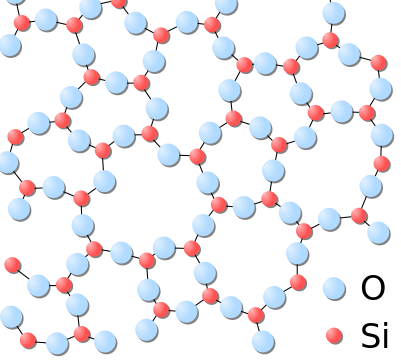
\includegraphics[width=3cm]{Cap_1/500px-Silica.png}
    \end{block}
  \end{column}
  \begin{column}{0.48\paperwidth}
    \tikz[na]{\node[coordinate] (n2) {};}
    \centering
    \begin{block}{Met\'alico}
      \centering Aleaci\'on met\'alica:\\
      Cu, Ni, Fe, Au, Zr, Be, La, Pd, Ti\\
      
      \vspace{0.2cm}
      Aunque tambi\'en puede contener no metales en baja concentraci\'on
    \end{block}
  \end{column}
\end{columns}

\begin{tikzpicture}[overlay]
        \path[->] (t1) edge [bend right] (n1);
        \path[->] (t2) edge [bend left] (n2);
\end{tikzpicture}

% \item Sus propiedades sobresalientes los hacen candidatos para aplicaciones modernas y de alta tecnolog\'ia. Material avanzado
\end{frame}

\definecolor{goodTitle}{HTML}{4D9A63}
\definecolor{goodDesc}{HTML}{A0DB8E}
\definecolor{alertTitle}{HTML}{FF2222}
\definecolor{alertDesc}{HTML}{FF9090}

\newcommand{\defaultBlocks}{
  \setbeamercolor{block title}{fg=white, bg=hsrmWarmGreyDark}
  \setbeamercolor{block body}{parent=palette secondary}
  \setbeamercolor{block title example}{fg=white, bg=hsrmSec1Dark}
  \setbeamercolor{block body example}{fg=white, bg=hsrmSec1}
  \setbeamercolor{block title alerted}{fg=white, bg=hsrmRedDark}
  \setbeamercolor{block body alerted}{fg=white, bg=hsrmRed}
}

\newcommand{\ventaja}[2]{
  \setbeamercolor{block title}{bg=goodTitle,fg=white}%
  \setbeamercolor{block body}{bg=goodDesc,fg=black}%
  \only<#1>{
    \begin{block}{Ventaja}%
    #2
    \end{block}%
   }
  \defaultBlocks%
}

\newcommand{\desventaja}[2]{
  \setbeamercolor{block title}{bg=alertTitle,fg=white}%
  \setbeamercolor{block body}{bg=alertDesc,fg=black}%
  \only<#1>{
    \begin{block}<#1>{Desventaja}%
    #2
    \end{block}%
  }
  \defaultBlocks%
}


\begin{frame}
\frametitle{Propiedades}
\begin{block}{¿Por qu\'e atrae el inter\'es de investigadores?}
 Combina propiedades de cer\'amicas y de metales a escala nanom\'etrica, resultando en un material de propiedades \'unicas
\end{block}
 
\ventaja{1}{{\begin{itemize}
             \item Alta dureza
             \item Resistencia al desgaste y la abrasi\'on
             \item Gran resistencia mec\'anica
             \item Alta resiliencia
            \end{itemize}
            }}

\end{frame}

\begin{frame}
\frametitle{Propiedades} 

\ventaja{1}{{\begin{itemize}
             \item Ausencia de efectos adversos debidos a fronteras de granos (resistencia a la corrosi\'on)
            \end{itemize}
            }}
\desventaja{1}{{\begin{itemize}
		\item Alto costo y grandes limitaciones de fabricaci\'on
		\item Gran p\'erdida de ductilidad ante la aparici\'on de bandas de corte
	      \end{itemize}
	      }}
            
\end{frame}

\begin{frame}
 \frametitle{Producci\'on}
 \vspace{-0.15cm}
 \begin{block}{}
    \textit{Te\'oricamente, todo l\'iquido podr\'ia convertirse en vidrio a velocidades de enfriamiento suficientemente altas y temperaturas suficientemente bajas evitando el proceso de cristalizaci\'on} (Turnbull et al, 1961)
 \end{block}
 
 %Las t\'ecnicas de fabricaci\'on act\'uan sobre la composici\'on, el volumen y la velocidad de enfriamiento
 \begin{textblock*}{10cm}(1.4cm,4.9cm)
  \begin{columns}
    \begin{column}{4cm}
      \begin{figure}
	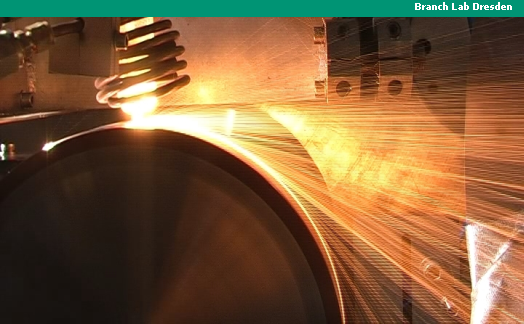
\includegraphics[width=4cm]{Cap_1/melt_spinning_B.png}
      \end{figure} 
      \begin{textblock*}{4cm}(1.3cm,8cm)
	\scriptsize{Proceso de \textit{Melt Spinnning}}
      \end{textblock*}
    \end{column}
    \begin{column}{6cm}
    \begin{alertblock}{Espesor}
	Los vidrios met\'alicos volum\'etricos, o \textit{Bulk Metallic Glasses} en ingl\'es, tienen una secci\'on transversal de por lo menos algunos mil\'imetros.
    \end{alertblock}
    \end{column}
  \end{columns}
 \end{textblock*}
 \begin{textblock*}{12.6cm}(0.5cm,9.2cm)
  \scriptsize{Turnbull, D. and Cohen, M., \textit{J. Chem. Phys.}, \textbf{34(1)}, 120-125 (1961)}
  \end{textblock*}
\end{frame}

\begin{frame}
 \frametitle{Mec\'anica de deformaci\'on}
 \begin{textblock*}{11.8cm}(0.5cm,1.8cm)
  \begin{block}{Bandas de corte}
  Concentraci\'on de deformaci\'on en bandas estrechas, llamadas \textbf{bandas de corte}.
  El crecimiento de estas bandas puede causar la fractura fr\'agil del material (Schuh et al, 2007).
  \end{block}
 \end{textblock*}
 \vspace{-0.7cm}
 \begin{textblock*}{\textwidth}(1cm,4.3cm)
  \begin{figure}
  \centering
  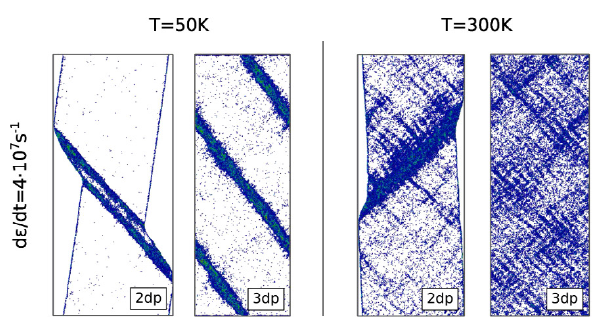
\includegraphics[width=5.5cm]{Cap_1/shearbands.png}
  \end{figure}
 \end{textblock*}
\begin{textblock*}{\textwidth}(1cm,8.2cm)
 \centering
 \scriptsize{Muestra de BMG bajo tracci\'on uniaxial. Adaptado de Albe et al, 2013}
\end{textblock*}

 \begin{textblock*}{12.6cm}(0.5cm,8.9cm)
 \scriptsize{Schuh, C., Hufnagel, T., and Ramamurty, U., \textit{Acta. Mater.}, \textbf{55(12)}, 4067-4109 (2007)} \\
 \scriptsize{Albe, K., Ritter, Y., and Şopu, D., \textit{Mech. Mater.}, \textbf{67}, 94–103 (2013)}
 \end{textblock*}

\end{frame}

\begin{frame}
 \frametitle{Aplicaciones}
 \centering
 Se trata de un material avanzado de ingenier\'ia
 
 \begin{textblock*}{12.6cm}(1.6cm,3cm)
  \begin{figure}
  \centering
  \begin{tabularx}{\textwidth}{cc}
  \only<1>{
    \subfloat[Joyer\'ia]{
      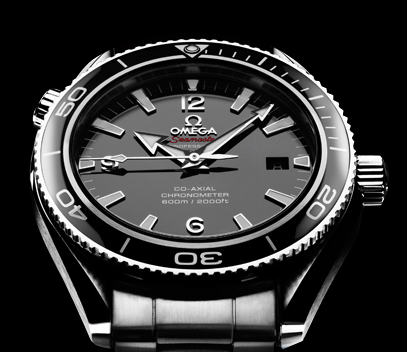
\includegraphics[height=3cm]{Cap_1/seamaster.png}}
    &
    \hspace{1cm}
    \subfloat[Deportes]{
      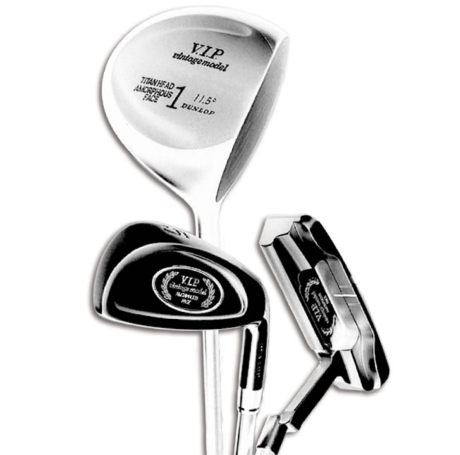
\includegraphics[height=3cm]{Cap_1/golf.png}}
    }
    \only<2>{
    \subfloat[MEMS]{
      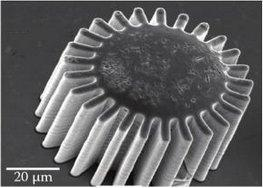
\includegraphics[height=3cm]{Cap_1/MEMS_A.jpeg}}
    &
    \subfloat[MEMS]{
      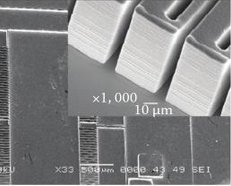
\includegraphics[height=3cm]{Cap_1/MEMS_B.jpeg}}
    }
    \only<3>{
     \subfloat[Filo est\'andar]{
      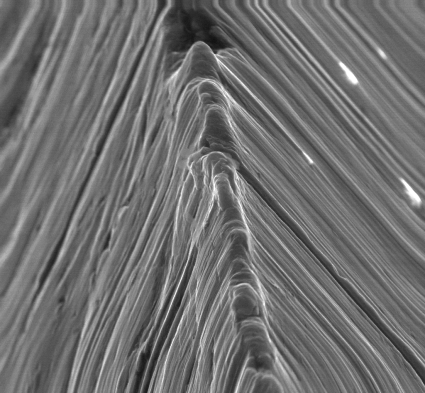
\includegraphics[height=3cm]{Cap_1/blade.png}}
      &
      \hspace{1cm}
      \subfloat[Filo de BMG]{
	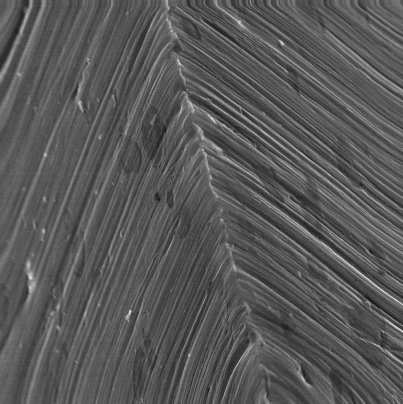
\includegraphics[height=3cm]{Cap_1/BMG-blade.png}}
    }
  \end{tabularx}
  \end{figure}
 \end{textblock*}
\end{frame}

\begin{frame}
 \frametitle{Objetivos}
 \vspace{0.5cm}
\begin{itemize}
 \item Investigar el comportamiento en r\'egimen elasto-pl\'astico en grandes deformaciones de un metal amorfo binario a diferentes temperaturas
 \begin{itemize}
  \item Tensión-deformación, parámetros constitutivos, dependencia con la temperatura.
 \end{itemize}
 \item Investigar los efectos de cambios en la composici\'on sobre las propiedades mec\'anicas
 \begin{itemize}
  \item Generar muestras modificadas: porosidad variable e inclusiones cristalinas
 \end{itemize}
\end{itemize}
\end{frame}

\begin{frame}
 \frametitle{Metodología}
 \begin{figure}
  \centering
  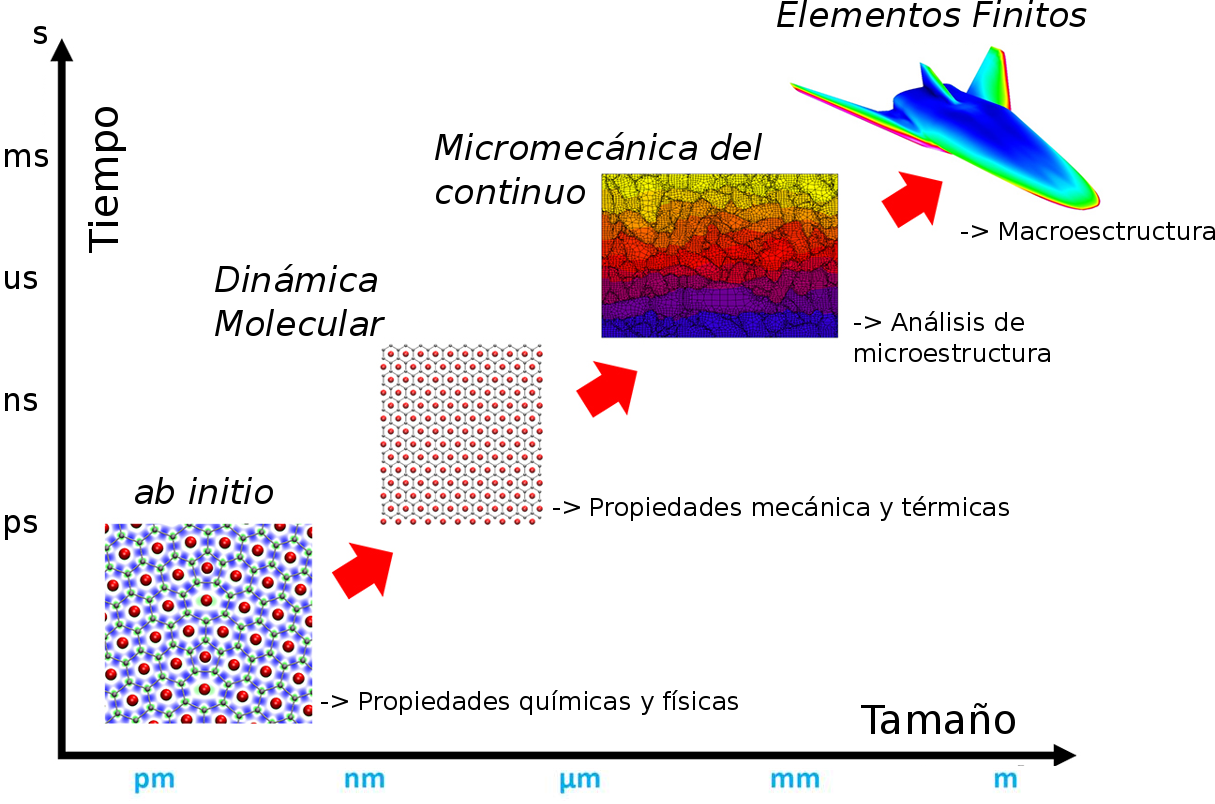
\includegraphics[width=10cm]{Presentacion/multiescala.png}
 \end{figure}

\end{frame}

\begin{frame}
 \frametitle{Metodología}
 %\vspace{0.5cm}
 \begin{block}{Simulaciones Din\'amica Molecular (MD)}
  Resuelve ecuaciones de Newton para un sistema de N mol\'eculas que interact\'uan seg\'un una funci\'on potencial
 \end{block}
 \begin{textblock*}{12cm}(1.1cm,4.9cm)
  Proceso de simulación:
  \begin{enumerate}
   \item Pre-procesamiento de la muestra.
   \item Preparación del script de simulación para LAMMPS.
   \item Secuenciación de tareas.
   \item Ejecución de LAMMPS.
   \item Generación de gráficas ''publication-ready''.
   \item Análisis estadístico, de Voronoi, y visual.
  \end{enumerate}
 \end{textblock*}
\end{frame}

%%%%%%%%%%%%%%%%%%%%%%%%%%%%%%%%%%%%%%%%%%%%%%%%%%%%%
%		CAP 3
%%%%%%%%%%%%%%%%%%%%%%%%%%%%%%%%%%%%%%%%%%%%%%%%%%%%%

\section[Caracterizaci\'on]{Caracterizaci\'on de un BMG}
\subsection{Caracterizaci\'on de un BMG}

\begin{frame}
    \frametitle{Introducci\'on}
    \vspace{0.2cm}
    \begin{block}{Objetivo}
     Entender el comportamiento mec\'anico a altas velocidades de deformaci\'on y distintas temperaturas
    \end{block}
    \vspace{1cm}
    \begin{itemize}
     \item T = 10, 100, 200, 300, 400, 500, 600, 900 K
     \item Condiciones de frontera periódicas en general
     \item Modos de carga: Uniaxial de tracción/compresión
    \end{itemize}

    %\vspace{1cm}
    %\begin{block}{Din\'amica molecular (MD)}
    %Resuelve ecuaciones de Newton para un sistema de N mol\'eculas que interact\'uan seg\'un una funci\'on potencial
    %\end{block}
\end{frame}

\begin{frame}
    \frametitle{Detalles de la simulaci\'on}
    \vspace{0.1cm}
    \begin{itemize}
        \item Software: LAMMPS (lammps.sandia.gov) para simulaci\'on, Ovito (www.ovito.org) para visualizaci\'on, Gnuplot/Shell/Python para an\'alisis
        \item Muestra: Cu$_{46}$Zr$_{54}$, descripta por Arman et al., 2010.
        \begin{itemize}
	  \item 160k \'atomos.
	  \item Velocidad de enfriamiento de 10$^{12}$K/s 
        \end{itemize}
	\item Velocidad de deformaci\'on: 10$^9$/s.
	\item Potencial EAM (embedded atom method; Daw,1984) ''alloy'' (Cheng, 2008).
    \end{itemize}
    \begin{textblock*}{12cm}(0.5cm,8cm) % {block width} (coords)
        \scriptsize{Arman B., Luo S.-N., Germann T.C. and Cağin T., \textit{Phys. Rev. B.}, \textbf{81}, 144201 (2010).\\
        Daw M. and Baskes M.I., \textit{Phys. Rev. B.}, \textbf{29}:6443-6453 (1984).\\
        Cheng Y.Q., Sheng H.W. and Ma E., \textit{Phys. Rev. B.}, \textbf{78}, 014207 (2008) https://sites.google.com/site/eampotentials/}
    \end{textblock*}
\end{frame}

\begin{frame}
    \frametitle{Resultados bajo condiciones peri\'odicas}
    \begin{textblock*}{12.6cm}(-0.08cm,1.5cm) 
      \begin{figure}[htp]
	\centering
	\subfloat[Tracci\'on]{
	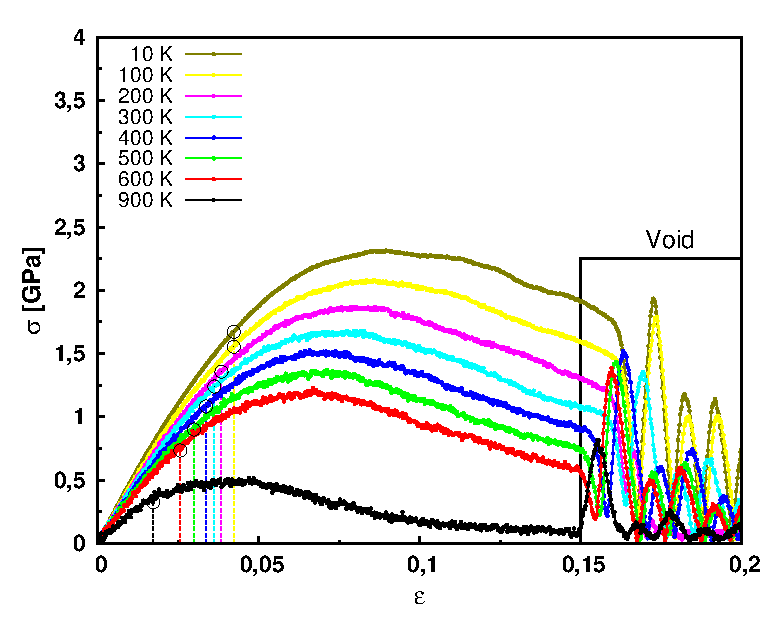
\includegraphics[width=6.3cm]{Presentacion_Mecom_2012/Tens_stress_strain_curve.eps}}
	\subfloat[Compresi\'on]{
	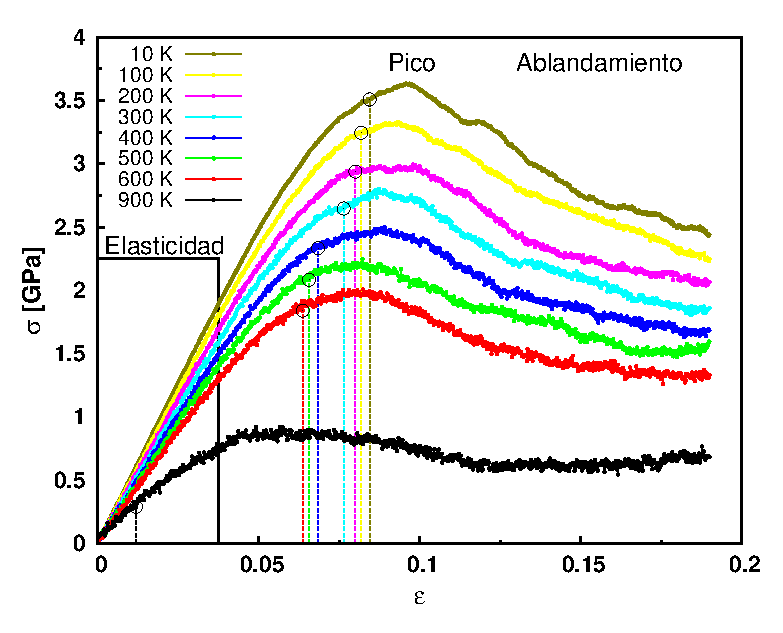
\includegraphics[width=6.3cm]{Presentacion_Mecom_2012/Comp_stress_strain_curve.eps}}
      \end{figure}
    \end{textblock*}
    \begin{textblock*}{6cm}(3.5cm,8cm) 
    \centering
      Tg=696 K\\
      (Glass transition temperature)
    \end{textblock*}
\end{frame}

\begin{frame}
 \frametitle{Resultados de las aproximaciones}
 \begin{textblock*}{6cm}(0.5cm,1.5cm) 
    
    \begin{table}[htp]
    \begin{center}
    \begin{tabular}{c c}
    \hline
    \textbf{Tracci\'on} & $R^{2}$ \\ \hline \hline
    $\sigma_{max}$ &  0.981 \\ \hline
    $\sigma$ ($\epsilon=0.12$) & 0.998 \\ \hline
    $E$ & 0.990 \\ \hline
    $\sigma_{y}$ &  0.972 \\ \hline
    \end{tabular}
    \end{center}
    \end{table}

    \begin{table}[htp]
    \begin{center}
    \begin{tabular}{*{4}{c}}
    \hline
    \textbf{Compresi\'on} & $R^{2}$ \\ \hline \hline
    $\sigma_{max}$ & 0.997 \\ \hline
    $\sigma$ ($\epsilon=0.18$) & 0.972 \\ \hline
    $E$ & 0.985 \\ \hline
    $\sigma_{y}$ & 0.985 \\ \hline
    \end{tabular}
    \end{center}
    \end{table}
 \end{textblock*}
  \begin{textblock*}{4.8cm}(7.7cm,2cm)
  \centering
   Para el c\'alculo de propiedades mec\'anicas, suponemos un comportamiento activado t\'ermicamente.
   \end{textblock*}
   \begin{textblock*}{4.8cm}(7.7cm,5cm)
   \centering
    $y=A_1^{(-T/T_0)}$
    \end{textblock*}
  \begin{textblock*}{4.8cm}(7.7cm,6cm)
  \centering
   El coeficiente de correlaci\'on es mayor a 0.9 en todos los casos, lo cual demuestra que la ecuaci\'on propuesta es razonable.
  \end{textblock*}
\end{frame}

\begin{frame}
 \frametitle{Gr\'aficos de las aproximaciones}
 \begin{textblock*}{10cm}(1.2cm,1.3cm)
 \begin{figure}[htp]
    \centering
    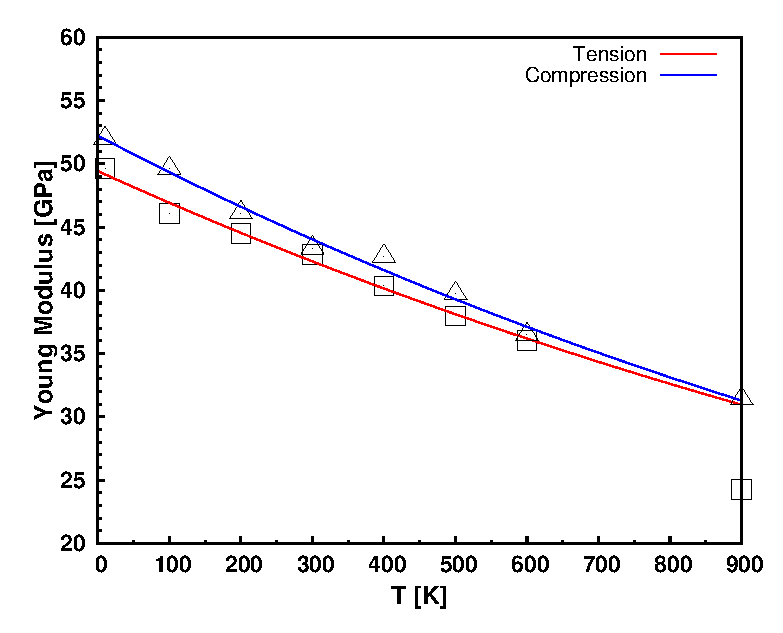
\includegraphics[width=4.5cm]{Presentacion_Mecom_2012/young_T_both.eps}
    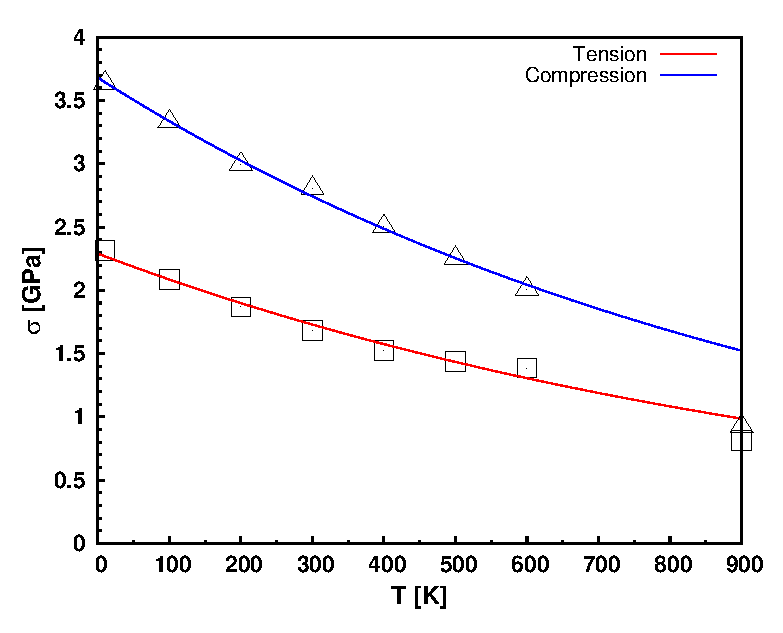
\includegraphics[width=4.5cm]{Presentacion_Mecom_2012/peakstress_T_BOTH.eps}
  \end{figure} 
 \end{textblock*}
 \begin{textblock*}{5cm}(1.5cm,4.9cm)
   \begin{figure}[htp]
    \centering
    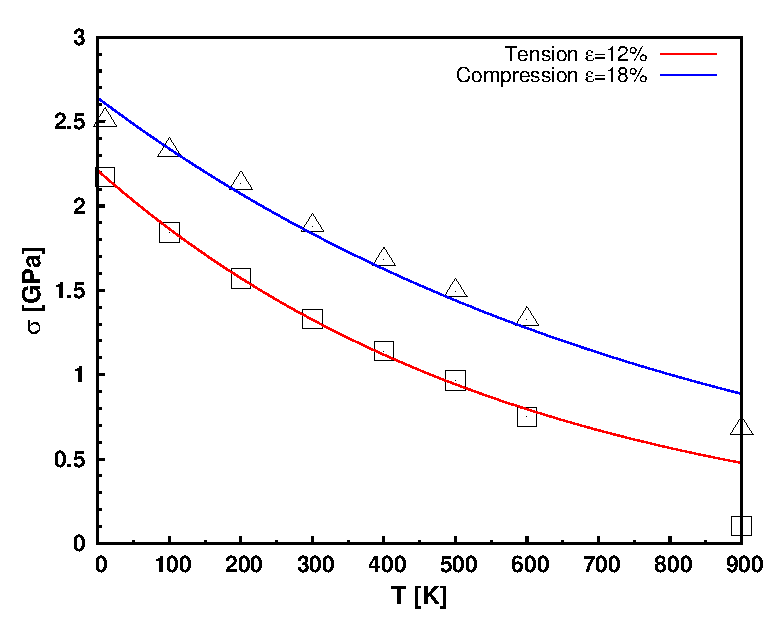
\includegraphics[width=4.5cm]{Presentacion_Mecom_2012/defstress_T_BOTH.eps}
  \end{figure} 
 \end{textblock*}
 \begin{textblock*}{5cm}(6.8cm,6.7cm)
  \centering
   Disminuci\'on de los valores con el aumento de temperatura.
  \end{textblock*}
\end{frame}

\begin{frame}
 \frametitle{Formaci\'on del void}
 \begin{figure}
    \centering
    \begin{tabular}{C{5cm} c}
      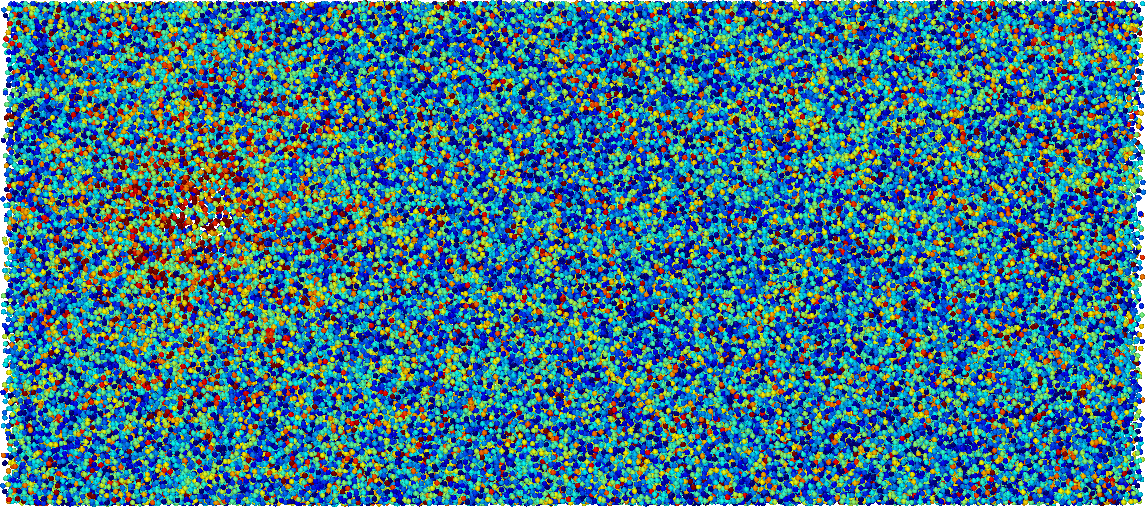
\includegraphics[width=5cm]{Cap_3/Poro_900_94000light_100-400.png} &  \multirow{3}{*}{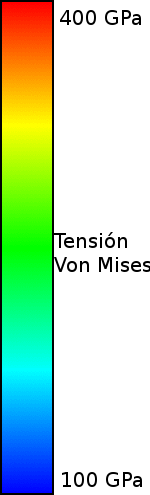
\includegraphics[width=1.2cm]{Cap_3/scale.png}}\\
      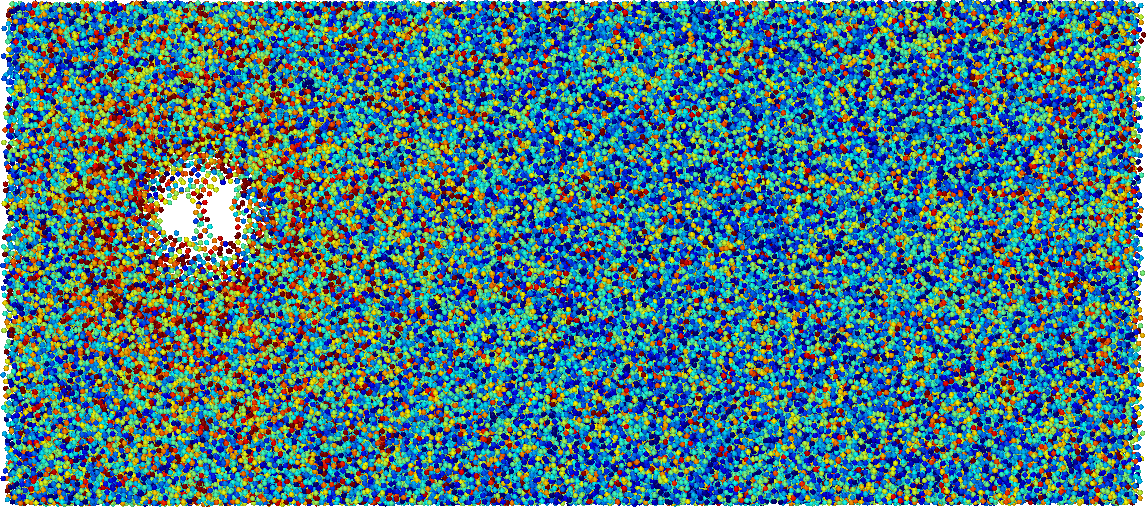
\includegraphics[width=5cm]{Cap_3/Poro_900_96000light_100-400.png} & \\
      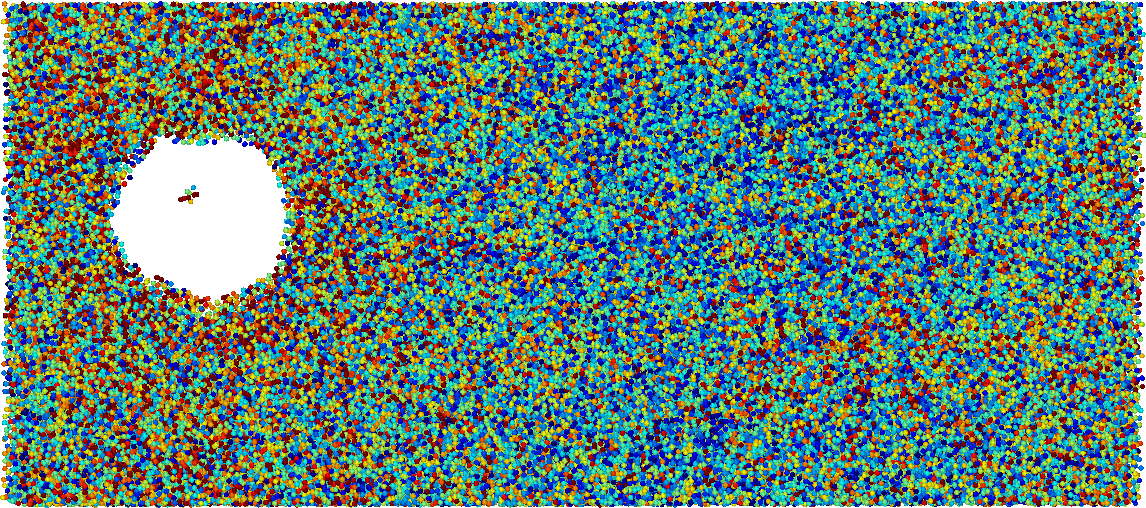
\includegraphics[width=5cm]{Cap_3/Poro_900_98000light_100-400.png} & \\
    \end{tabular}
    \label{C3:fg:voidSeq}
  \end{figure}
  \begin{textblock*}{2cm}(1cm,3cm)
      $\epsilon=14.4\%$
  \end{textblock*}
  \begin{textblock*}{2cm}(1cm,5.5cm)
    $\epsilon=14.6\%$
  \end{textblock*}
  \begin{textblock*}{2cm}(1cm,8cm)
    $\epsilon=14.8\%$
  \end{textblock*}
  \begin{textblock*}{4cm}(8.5cm,2.5cm)
    Temperatura 900K
  \end{textblock*}
\end{frame}

\begin{frame}
 \frametitle{Comportamiento pl\'astico}
 \begin{textblock*}{7cm}(0.5cm,1.4cm)
  \begin{figure}[htp]
      \centering
      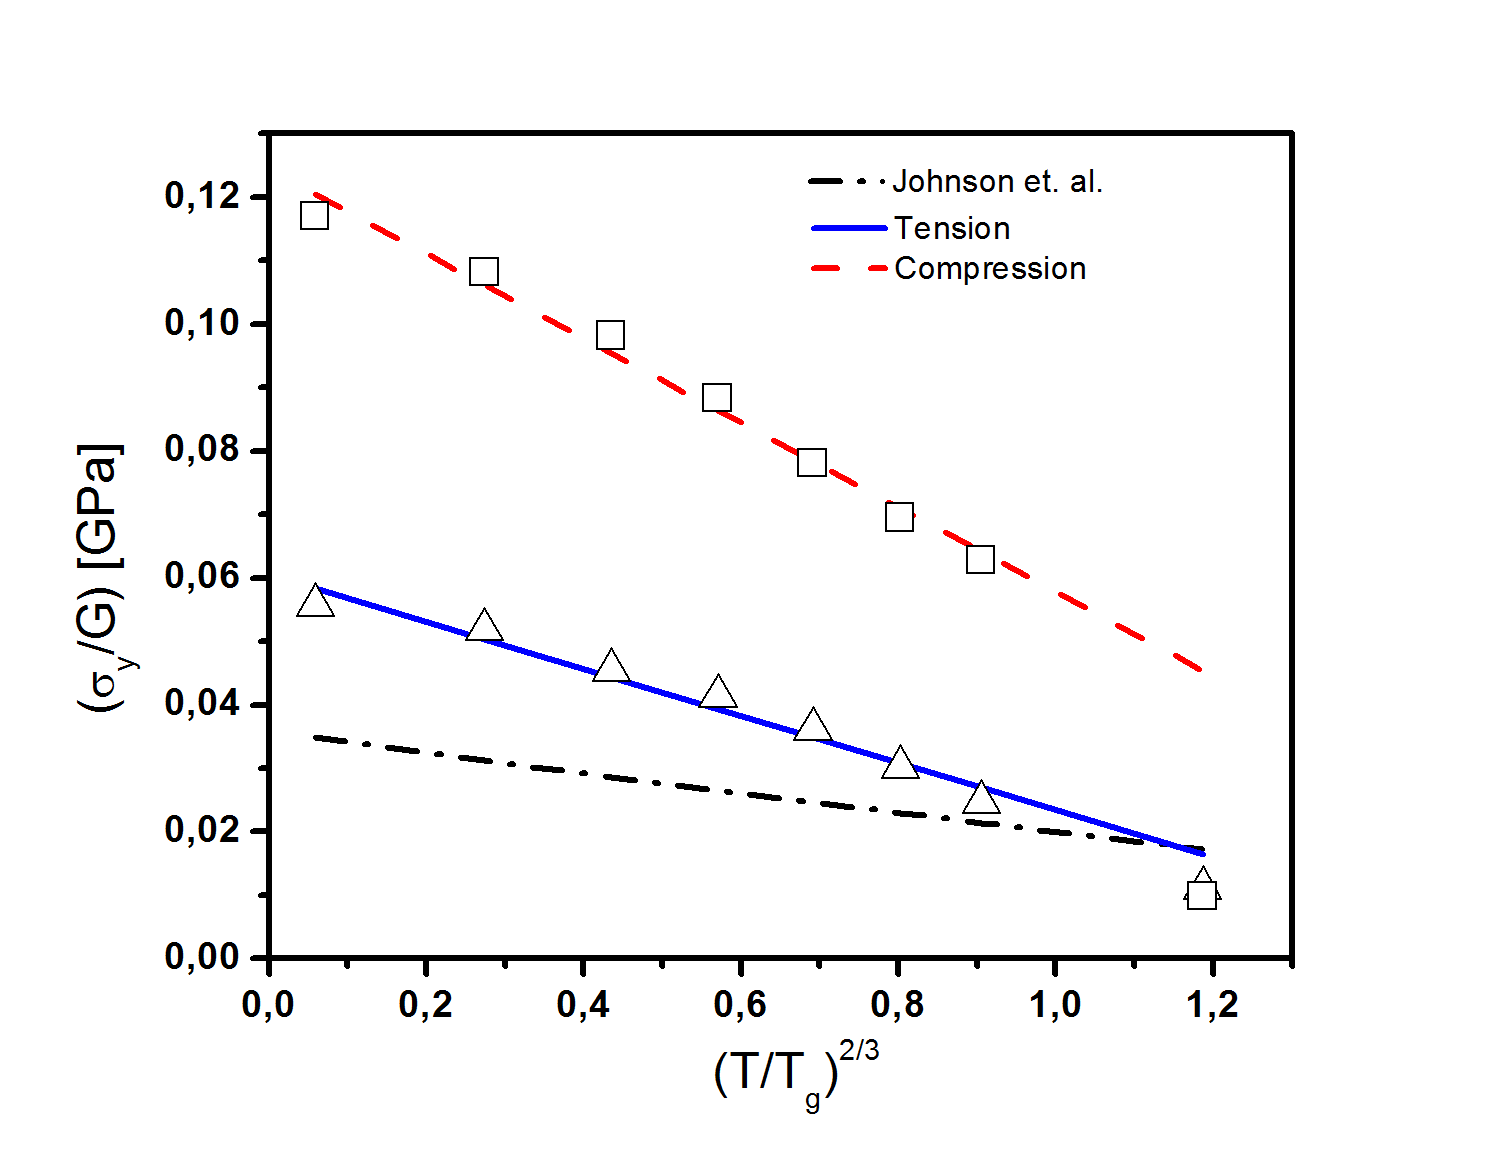
\includegraphics[width=7cm]{Cap_3/Fit2_Tercios.png}
  \end{figure}
 \end{textblock*}
 \begin{textblock*}{4.5cm}(8cm,2.5cm)
      Expresi\'on adaptada de Cheng et al. (2011) :\\
	$\sigma_y/G =A+B(T/T_g)^{2/3}$
  \end{textblock*}
  \begin{textblock*}{4.5cm}(8cm,4.5cm)
      Valores normalizados mediante:
      \begin{itemize}
       \item $T_g=696K$
       \item $G=30GPa$
      \end{itemize}
      \footnotesize{(Johnson y Samwer, 2005)}
  \end{textblock*}
  \begin{textblock*}{5cm}(2cm,7.5cm)
    \scriptsize{Esfuerzo de fluencia vs. temperatura}
  \end{textblock*}
  \begin{textblock*}{12cm}(0.5cm,8.5cm) % {block width} (coords)
    \scriptsize{Cheng Y.Q. and Ma E., \textit{Acta Mater.}, \textbf{59}, 1800-1807 (2011).\\
    Johnson W.L., Samwer K., \textit{Phys. Rev. Lett.}, \textbf{95}, 195501 (2005).}
  \end{textblock*}
\end{frame}

\begin{frame}
  \frametitle{Muestras}
  \begin{textblock*}{6cm}(0.5cm,1.5cm)
    \begin{figure}[htp]
      \centering
      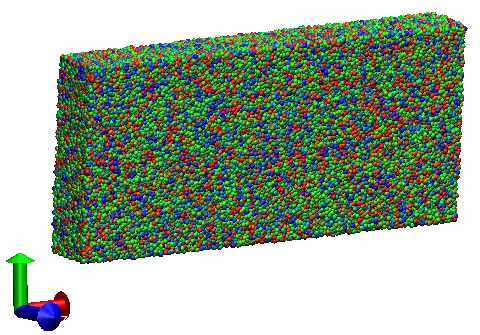
\includegraphics[width=6cm]{Cap_3/All_300K_6pstrain_sacale100-280_Trac.png}
    \end{figure}
  \end{textblock*}
  \begin{textblock*}{6cm}(6.5cm,4cm)
    \begin{figure}[htp]
      \centering
      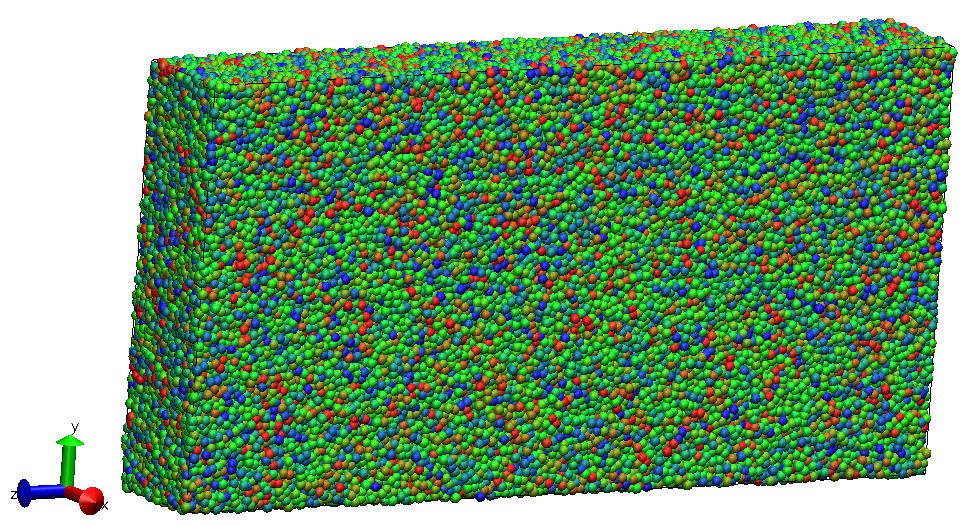
\includegraphics[width=6cm]{Cap_3/All_300K_6pstrain_sacale100-400_Comp.png}
    \end{figure}
  \end{textblock*}
  \begin{textblock*}{4cm}(3cm,6.2cm)
   \scriptsize{Tracci\'on. $T=300K$. $\epsilon=6\%$}
  \end{textblock*}
  \begin{textblock*}{5cm}(8cm,8.5cm)
   \scriptsize{Compresi\'on. $T=300K$. $\epsilon=6\%$}
  \end{textblock*}
  \begin{textblock*}{5cm}(7cm,2.5cm)
   \centering
   La escala de colores representa la tensi\'on de Von Mises
  \end{textblock*}
  \begin{textblock*}{5cm}(1cm,7.5cm)
   \centering
   No se observan bandas de corte
  \end{textblock*}
\end{frame}

\begin{frame}
  \frametitle{Deformaci\'on at\'omica}
  \begin{textblock*}{4cm}(4.5cm,1.5cm)
    \begin{figure}[htp]
      \centering
      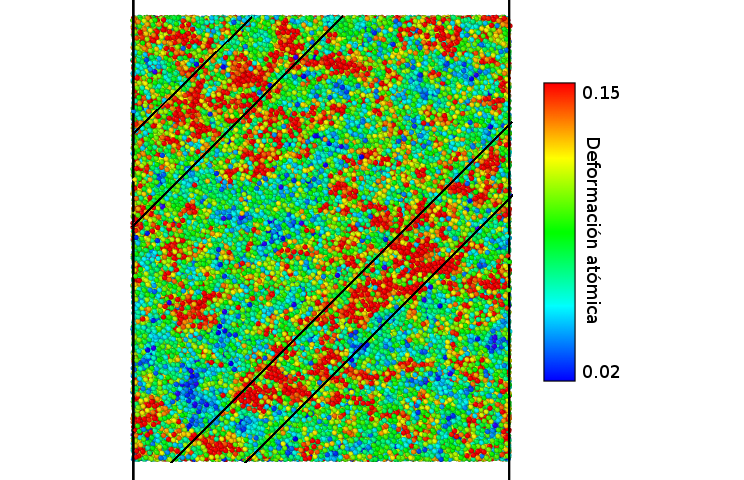
\includegraphics[height=6cm]{Cap_3/ShearBand.png}
    \end{figure}
  \end{textblock*}
  \begin{textblock*}{5cm}(6.5cm,8.5cm)
   \scriptsize{Compresi\'on. $T=300K$. $\epsilon=14\%$}
  \end{textblock*}
  \begin{textblock*}{5cm}(0.5cm,3cm)
   \centering
   La escala de colores representa deformaci\'on at\'omica
  \end{textblock*}
  \begin{textblock*}{5cm}(0.5cm,5.5cm)
   \centering
   Hay bandas de corte incipientes que se forman con una direcci\'on predominantemente diagonal
  \end{textblock*}
  
\end{frame}

\begin{frame}
  \frametitle{Resultados bajo condiciones libres}
  
  \begin{textblock*}{5cm}(0.5cm,1.2cm)
    \begin{figure}[htp]
      \centering
      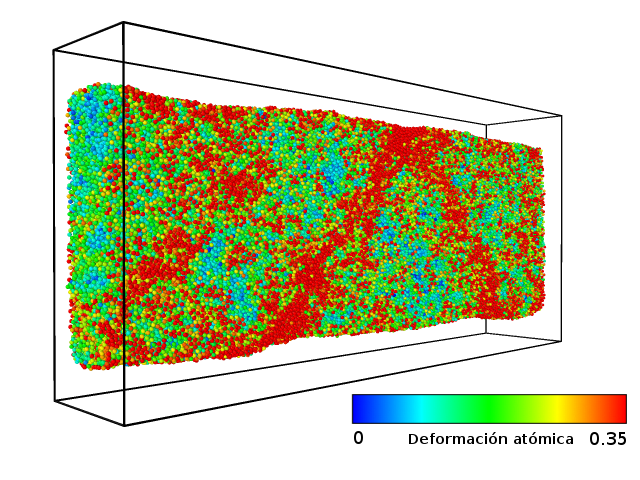
\includegraphics[width=5cm]{Cap_3/Pseudo_Free_Boundaries_ShearStrain_0_035_300K_20strain.png}
    \end{figure}
  \end{textblock*}
  
  \only<1>{
  \begin{textblock*}{5cm}(6.5cm,1.2cm)
    \begin{figure}[htp]
      \centering
      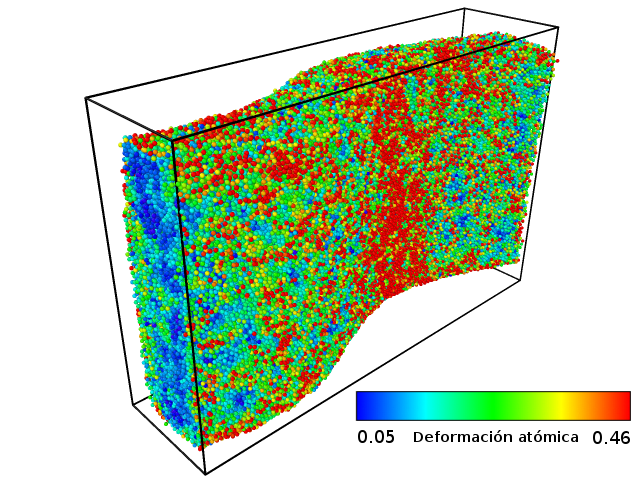
\includegraphics[width=5cm]{Cap_3/Pseudo_Free_Boundaries_ShearStrain_005_046_300K_15strain.png}
    \end{figure}
  \end{textblock*}
  }
  
  \begin{textblock*}{4cm}(2.3cm,5.5cm)
   \scriptsize{Tracci\'on. $T=300K$. $\epsilon=20\%$}
  \end{textblock*}
  
  \only<1>{
  \begin{textblock*}{4cm}(8.7cm,5.5cm)
   \centering
   \scriptsize{Compresi\'on. $T=300K$. $\epsilon=15\%$}
  \end{textblock*}
  }
  
  \begin{textblock*}{7cm}(0cm,6.5cm)
   \centering
   \small{Existe un cambio de la secci\'on transversal en tracci\'on.}
  \end{textblock*}
  \begin{textblock*}{9cm}(0cm,7.7cm)
   \centering
   \small{Son similares a las de nanoalambres de vidrios met\'alicos vistas en Xiao et al. (2012).\\}
  \end{textblock*}
  
  \only<1>{
  \begin{textblock*}{3cm}(8.5cm,5.5cm)
    \begin{figure}[htp]
	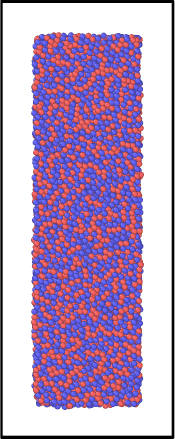
\includegraphics[width=1.3cm]{Cap_3/Pseudo_Free_Boundaries_0strain_transversal.png}
	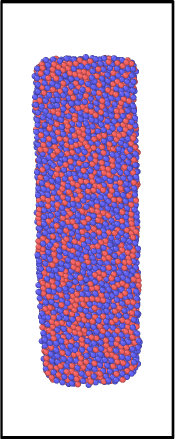
\includegraphics[width=1.3cm]{Cap_3/Pseudo_Free_Boundaries_20strain_transversal_esquina.png}
    \end{figure}
  \end{textblock*}
  }
  
  \only<2>{
  \begin{textblock*}{2cm}(9.7cm,2cm)
    \begin{figure}[htp]
	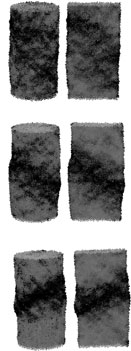
\includegraphics[width=2cm]{Presentacion_Mecom_2012/XiaoNanowire.png}
    \end{figure}
  \end{textblock*}
  
  \begin{textblock*}{12cm}(0.5cm,9cm)
    \scriptsize{Xiao Q., Sheng H.W. and Shi Y., \textit{MRS Commun.}, \textbf{2}, 13-16 (2012)}
  \end{textblock*}

  \begin{textblock*}{2cm}(7.7cm,3.1cm)
    \centering
    \scriptsize{$1.7\cdot10^{12}K/s$}
  \end{textblock*}
  
  \begin{textblock*}{2cm}(7.7cm,4.9cm)
    \centering
    \scriptsize{$1.7\cdot10^{11}K/s$}
  \end{textblock*}
  
  \begin{textblock*}{2cm}(7.7cm,6.8cm)
    \centering
    \scriptsize{$1.7\cdot10^{10}K/s$}
  \end{textblock*}
  
  }
\end{frame}
%%%%%%%%%%%%%%%%%%%%%%%%%%%%%%%%%%%%%%%%%%%%%%%%%%%%%
%		CAP 4
%%%%%%%%%%%%%%%%%%%%%%%%%%%%%%%%%%%%%%%%%%%%%%%%%%%%%

\section[BMG con nanopart\'iculas]{BMG con nanopart\'iculas embebidas}
\subsection{BMG con nanopart\'iculas embebidas}

\begin{frame}
  \frametitle{Introducci\'on}
  \begin{textblock*}{12.6cm}(0cm,1.2cm)
    \begin{figure}
    \centering
    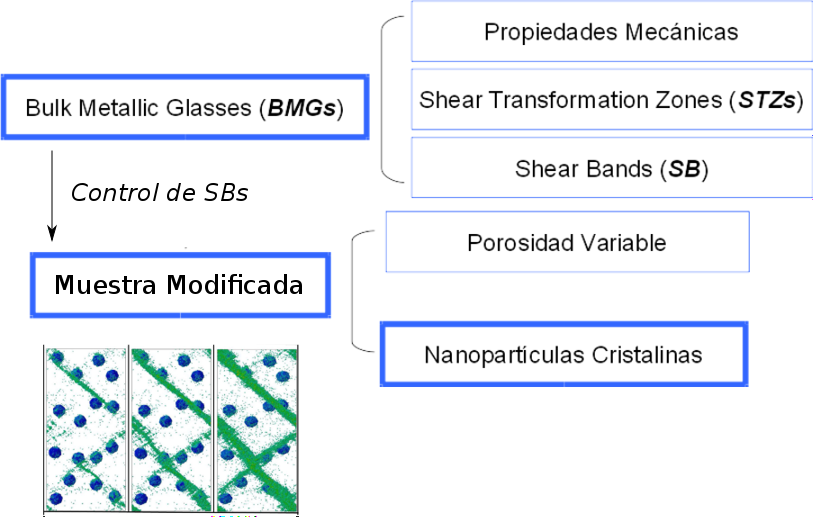
\includegraphics[width=11cm]{Presentacion/modifications_A.png}
    \end{figure}
  \end{textblock*}

%   \begin{itemize}
%    \item Para homogeneizar el r\'egimen pl\'astico y evitar la falla fr\'agil del material, la composici\'on se modifica de diferentes maneras
%   \end{itemize}
%   \begin{textblock*}{12.6cm}(-0.1cm, 3cm)  
%     \begin{figure}[htp]
%       \centering
%       \begin{tabular}{c}
% 	\subfloat[Nanopart\'iculas (Albe et al, 2013)]{
% 		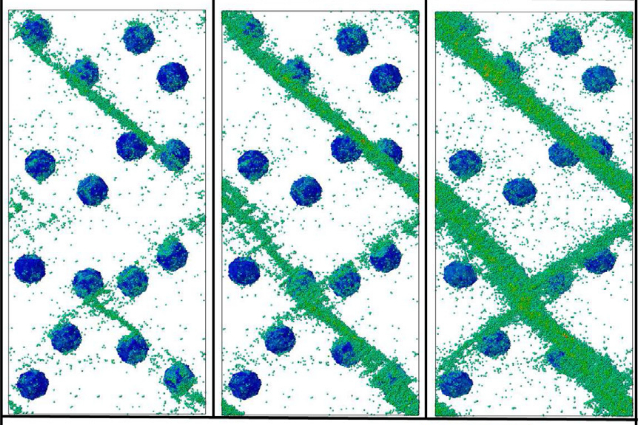
\includegraphics[width=5.7cm]{Presentacion/nanoparticles_example.png}
% 		\label{P:fg:B2Crystal}}
% 	\hspace{0.5cm}
% 	\subfloat[Nanovidrios (Adibi et al, 2013)]{
% 		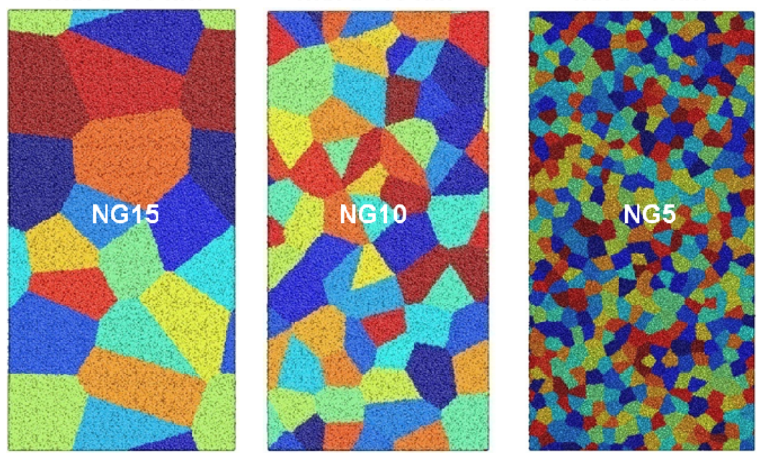
\includegraphics[width=6cm]{Presentacion/nanoglass_example.png}
% 		\label{P:fg:B2CrystalTest}}
%       \end{tabular}
%     \end{figure}
%   \end{textblock*}
  \begin{textblock*}{4.5cm}(5.5cm,8.3cm)
  \scriptsize{Albe, K., Ritter, Y., and Şopu, D., \textit{Mech. Mater.}, \textbf{67}, 94–103 (2013)}
%   Adibi, S., Sha, Z., Branicio, P., Joshi, S., Liu, Z., and Zhang, Y., \textit{Appl. Phys. Lett.}, \textbf{103}, 211905 (2013).\\
  \end{textblock*}
\end{frame}

\begin{frame}
\frametitle{Objetivos del estudio}
\vspace{0.5cm}
 \vspace{0.5cm}
 \begin{itemize}
  \item Estabilidad t\'ermica de las nanopart\'iculas (difusi\'on del material cristalino en la matriz amorfa).
  \vspace{0.5cm}
  \item Impacto en el comportamiento mec\'anico de la muestra (cambios en curvas tensi\'on-deformaci\'on)
  \vspace{0.5cm}
  \item Distribuci\'on de la deformaci\'on at\'omica de la muestra.
 \end{itemize}
\end{frame}

\begin{frame}
 \frametitle{Detalles de la simulaci\'on}
 \vspace{0.3cm}
 \begin{itemize}
  \item Muestra original ya caracterizada: Cu$_{46}$Zr$_{54}$ - 160k \'atomos
  \item Condiciones de bordes peri\'odicas en las tres dimensiones
  \item Nanopart\'iculas: Esferas de 2 nm de radio de composici\'on (a) Cu-FCC y (b) CuZr-B2
  \item La constante de red del cobre se establece en 0.3615 nm
  \item La estructura CuZr-B2 se genera ad-hoc para la simulaci\'on y da como resultado una constante de 0.3283 nm
  \item Velocidad de deformaci\'on de 10$^{9}$/s
 \end{itemize}
\end{frame}

% \begin{frame}
%  \frametitle{Preparaci\'on de cristal CuZr-B2}
%   \begin{itemize}
%     \item Cubo cristalino aislado de 15 celdas unitarias de ancho
%     \item Constante de celda de 3.50 \AA{} \cite{inoue04}
%     \item PBC en las tres dimensiones
%     \item Minimizado de energ\'ia y relajaci\'on a presi\'on cero.
%     \item T$_{i}$ = 1100 K \cite{pauly10} (988 K $\leq$ T$_{B2}$ $\leq$ 1200 K)
%     \item Se equilibra a P = 0 y T = T$_{B2}$ en 100 ps
%     \item Recocido a T = T$_{B2}$ por 150 ps
%     \item Enfriado r\'apido a 10$^{12}$ K/s hasta 300 K
%   \end{itemize}
% \end{frame}
% \begin{frame}
%   \frametitle{Preparaci\'on de cristal CuZr-B2}
%   \begin{textblock*}{12cm}(0cm,3cm)
%     \begin{table}[htp]
%     \begin{center}
%     \begin{tabular}{*{2}{c}}
%     \hline
%     Velocidad de enfriamiento [K/s] & 10$^{12}$ \\
%     \hline
%     N\'umero de \'atomos & 6750 \\
%     \hline
%     Constante de celda [\AA] & 3.283 \\
%     \hline
%     Energ\'ia total (eV) & -34012.8 \\
%     \hline
%     Energ\'ia de cohesi\'on (eV) & -5.04 \\
%     \hline
%     \end{tabular}
%     \end{center}
%     \end{table}
%   \end{textblock*}
%   
%   \begin{textblock*}{12cm}(0cm,7cm) 
%     \centering
%       Par\'ametros obtenidos para el cristal CuZr (B2)
%   \end{textblock*}
% \end{frame}
\begin{frame}
  \frametitle{Preparaci\'on de cristal CuZr-B2}
    \begin{textblock*}{12.6cm}(-0.08cm,1.5cm) 
      \begin{figure}[htp]
	\centering
	\subfloat[Cristal]{
	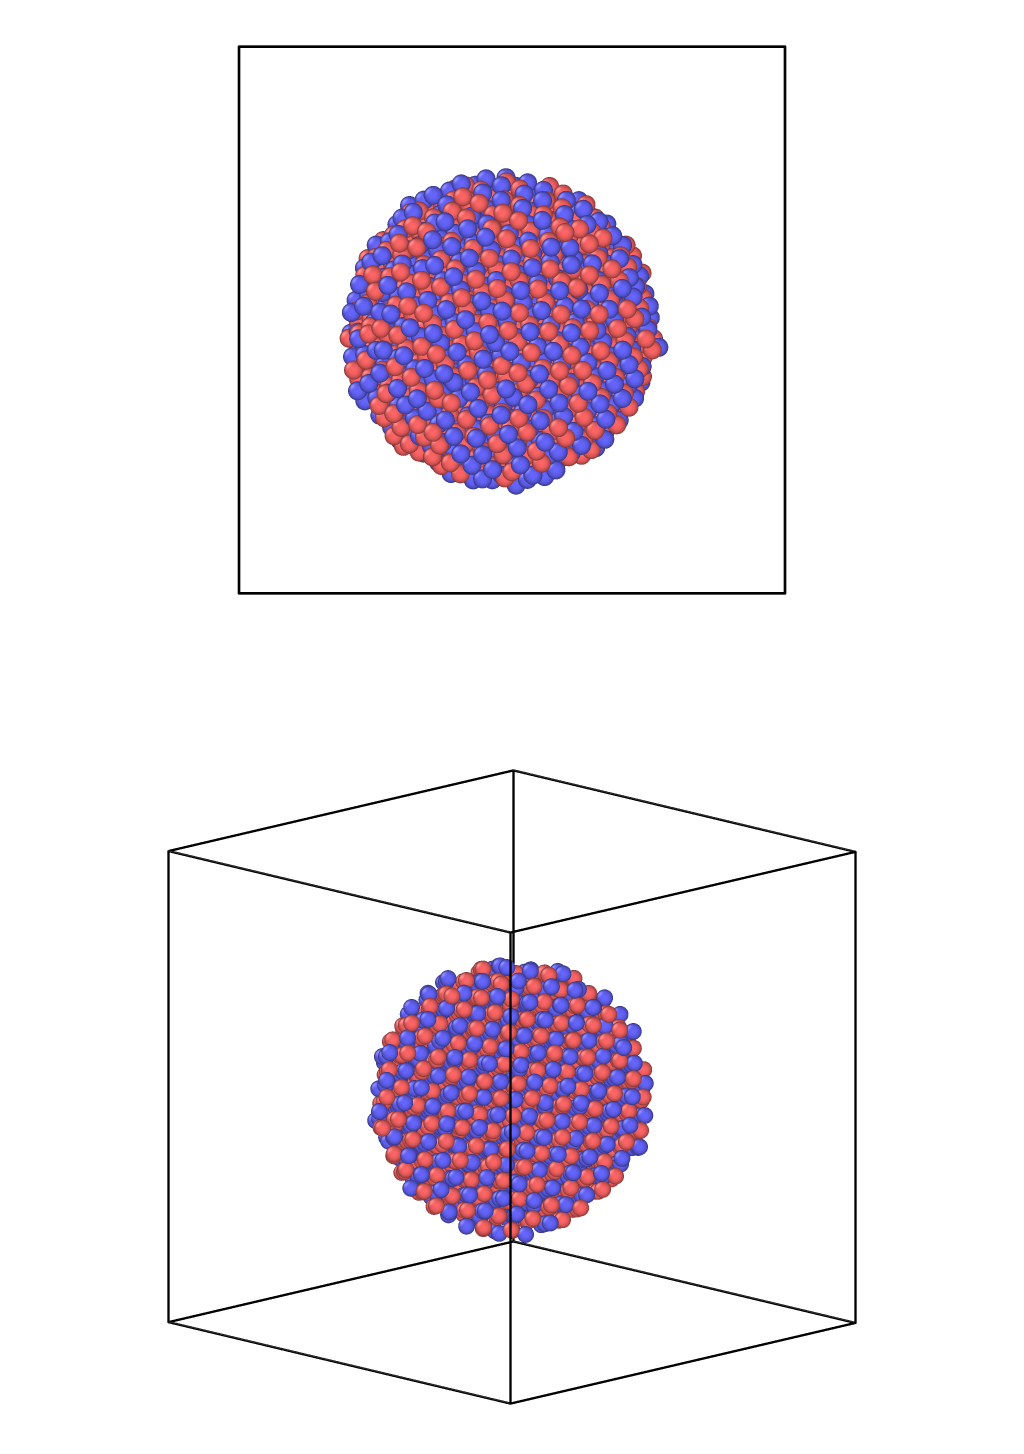
\includegraphics[height=5cm]{Cap_4/B2_FreeBoundaries.png}}
	\subfloat[Energ\'ia de cohesi\'on vs tiempo]{
	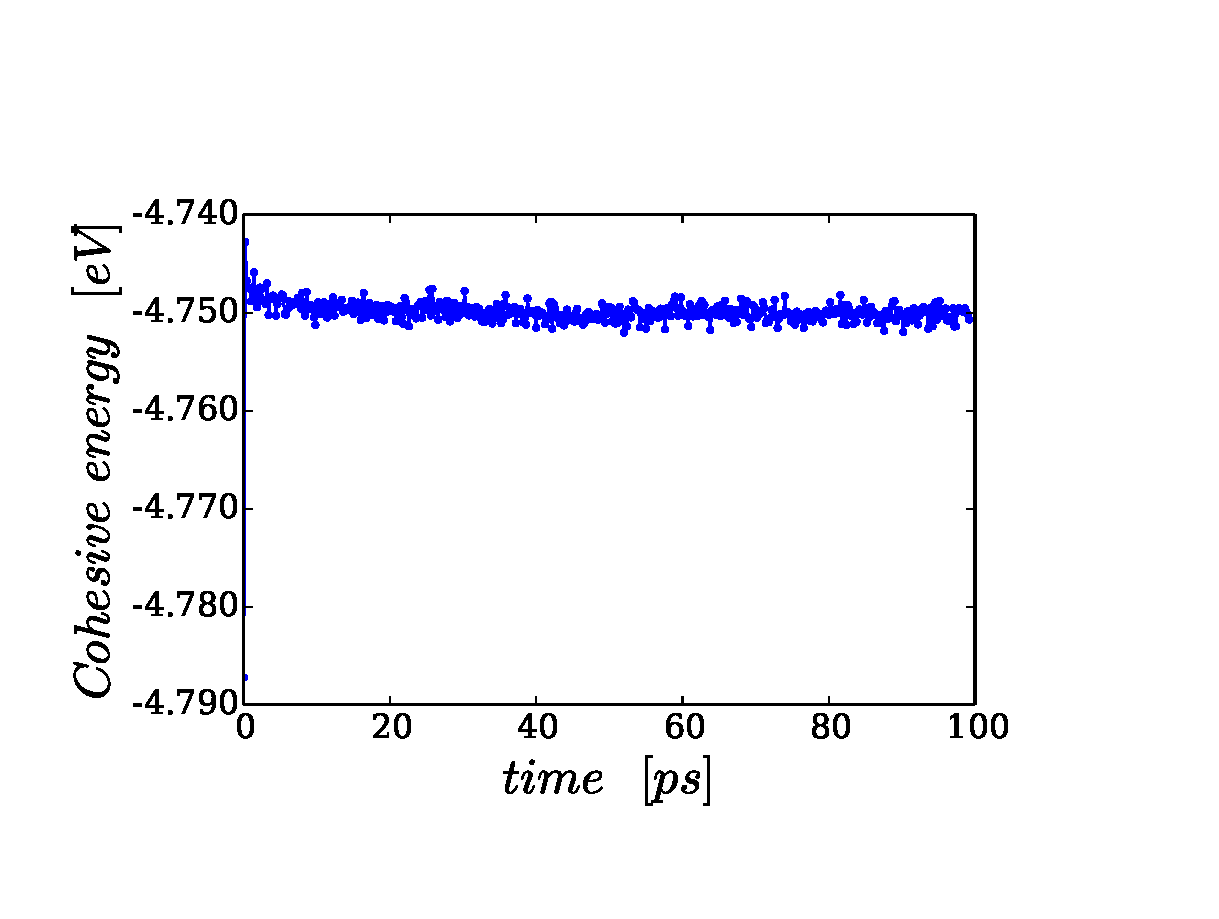
\includegraphics[width=6.3cm]{Cap_4/B2CrystalTest_FreeBoundariesSphere.pdf}}
      \end{figure}
    \end{textblock*}
    \begin{textblock*}{10cm}(1.5cm,8.5cm) 
    \centering
      Verificaci\'on del cristal CuZr-B2
  \end{textblock*}
\end{frame}

% \begin{frame}
%  \frametitle{Vista de la muestra preparada}
%  
%  \begin{textblock*}{12.6cm}(-0.08cm,1.5cm) 
%      \begin{figure}[htp]
% 	\centering
% 	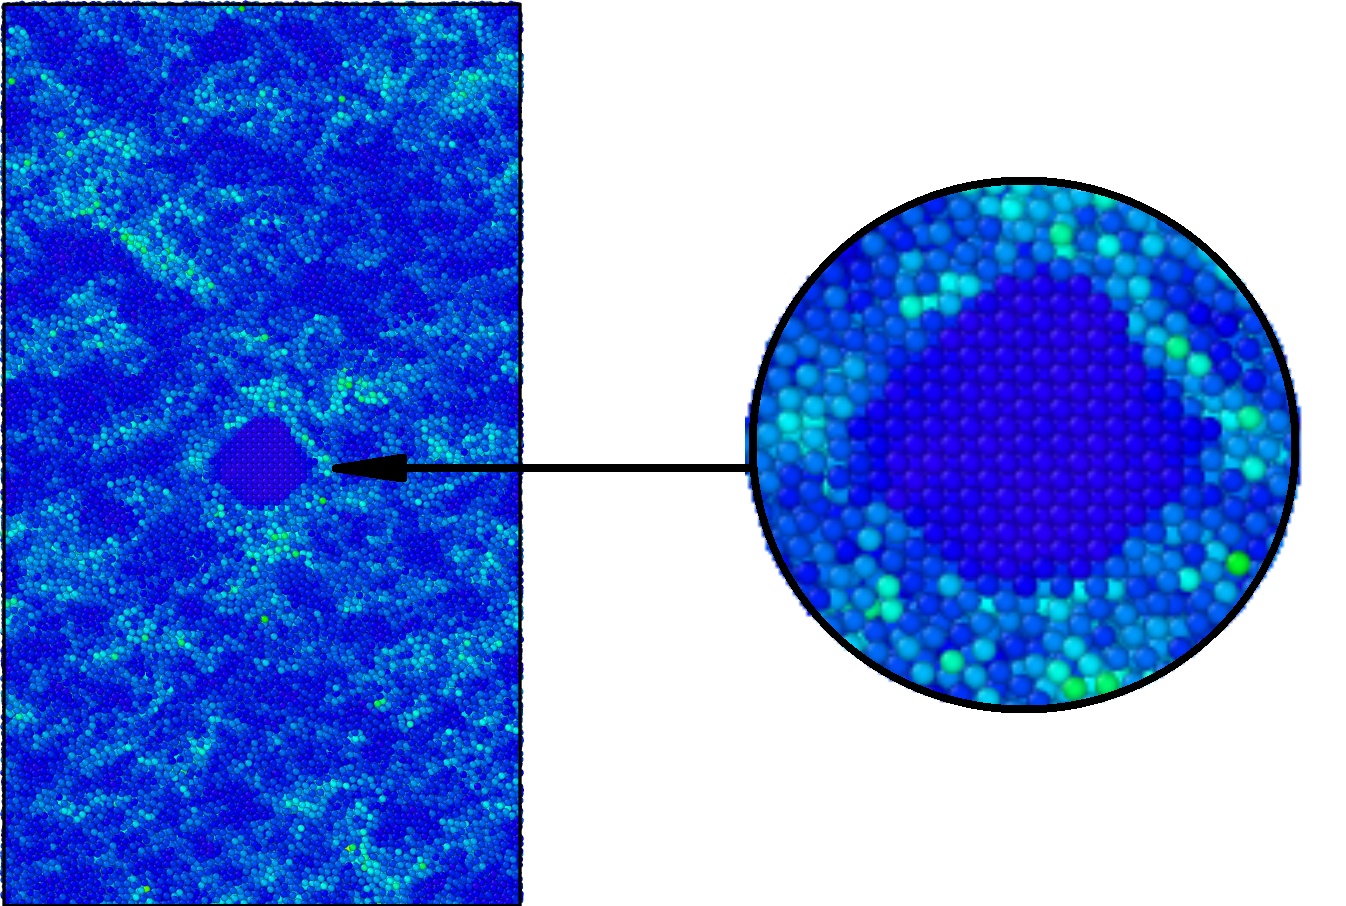
\includegraphics[height=6cm]{Cap_4/NP_CloseUp_FCC.png}
%       \end{figure}
%   \end{textblock*}
%  
% \end{frame}

\begin{frame}
 \frametitle{Resultados}
 
 \begin{textblock*}{12.6cm}(-0.08cm,1.5cm) 
      \begin{figure}[htp]
	\centering
	\subfloat[Bajas Temperaturas]{
	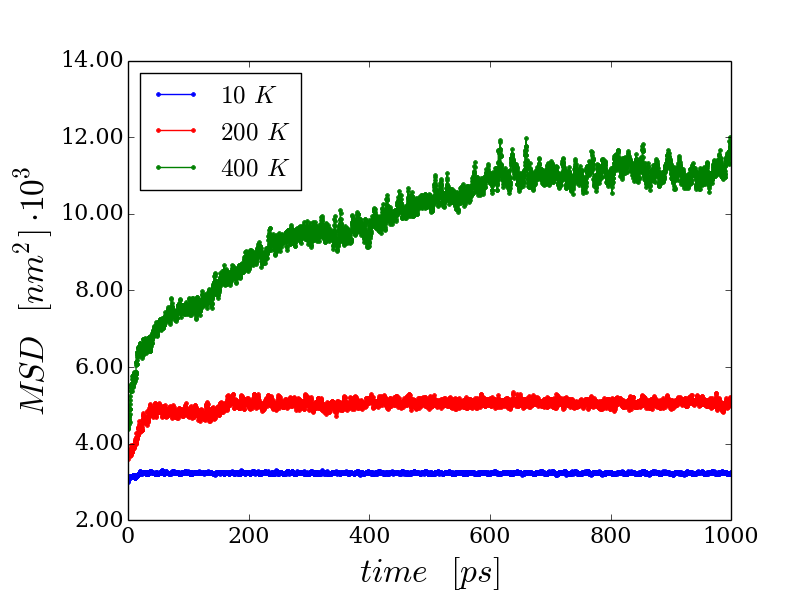
\includegraphics[width=6.3cm]{Cap_4/msd10_400_FCC.png}}
	\subfloat[Altas Temperaturas]{
	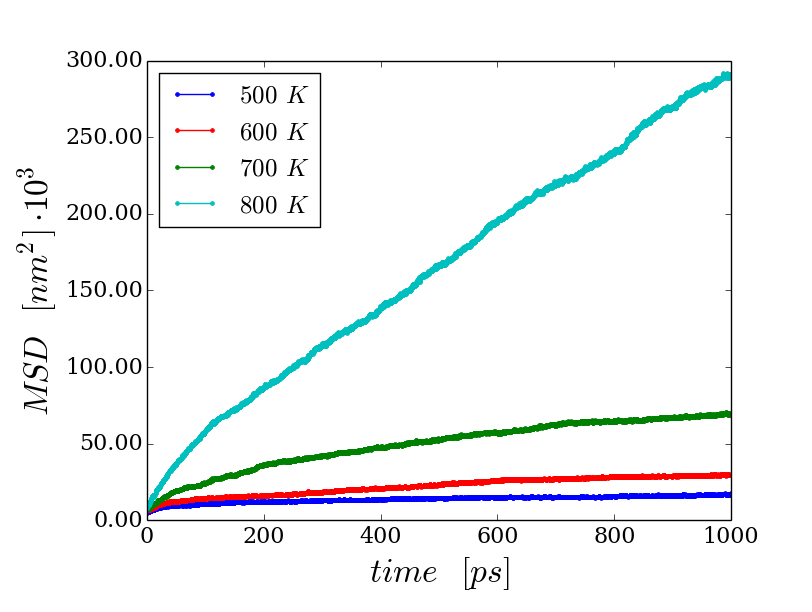
\includegraphics[width=6.3cm]{Cap_4/msd500_800_FCC.png}}
      \end{figure}
    \end{textblock*}
    \begin{textblock*}{10cm}(1.5cm,8cm) 
    \centering
      Desplazamientos cuadr\'aticos medios para la nanopart\'icula Cu-FCC
 \end{textblock*}
\end{frame}

\begin{frame}
 \frametitle{Resultados}
 
 \begin{textblock*}{12.6cm}(-0.08cm,1.5cm) 
      \begin{figure}[htp]
	\centering
	\subfloat[Bajas Temperaturas]{
	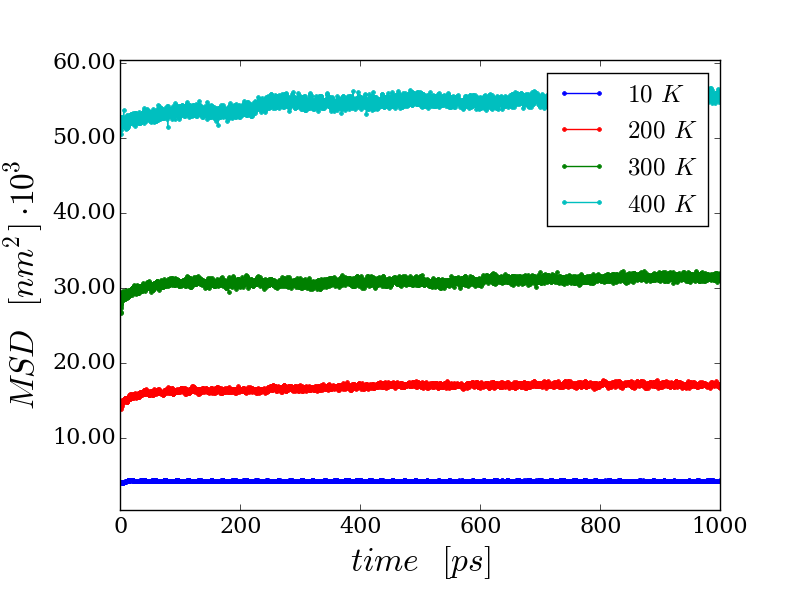
\includegraphics[width=6.3cm]{Cap_4/msd10_400_B2.png}}
	\subfloat[Altas Temperaturas]{
	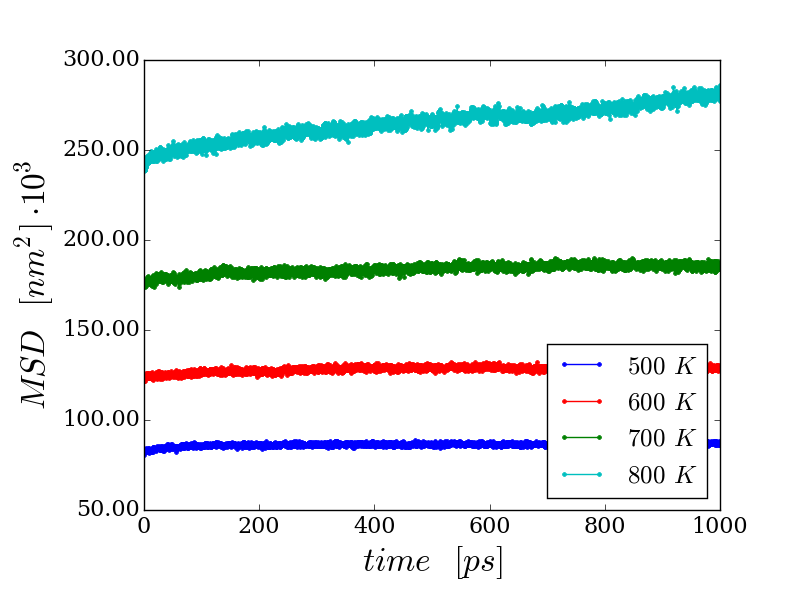
\includegraphics[width=6.3cm]{Cap_4/msd500_800_B2.png}}
      \end{figure}
    \end{textblock*}
    \begin{textblock*}{10cm}(1.5cm,8cm) 
    \centering
      Desplazamientos cuadr\'aticos medios para la nanopart\'icula CuZr-B2
 \end{textblock*}
\end{frame}

\begin{frame}
 \frametitle{Resultados}
 
  \begin{textblock*}{6.5cm}(-0.08cm,2cm) 
   \begin{figure}[htp]
    \centering
    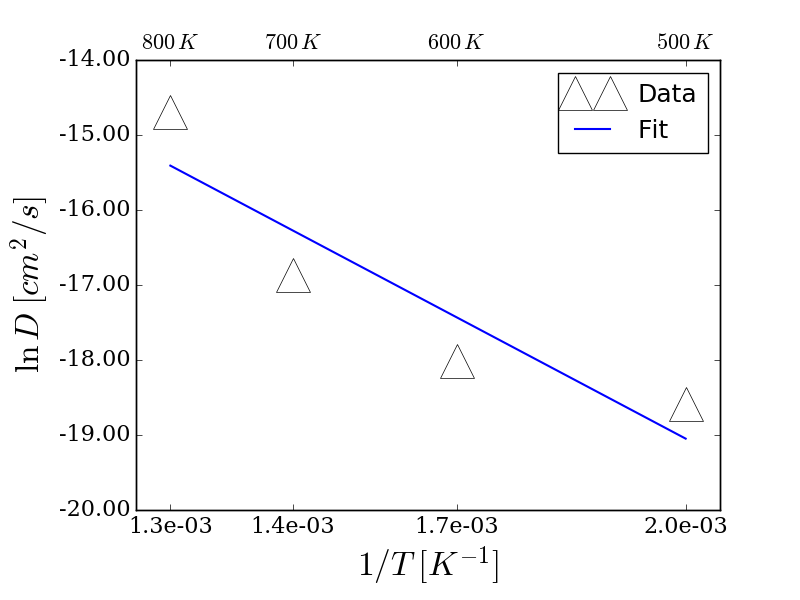
\includegraphics[width=6.3cm]{Cap_4/FCCDiff_vs_temp_fit.png}
   \end{figure}
  \end{textblock*}
  \begin{textblock*}{12cm}(0.2cm,8.5cm) 
    \centering
    Difusividad en funci\'on de la temperatura para el caso Cu-FCC
  \end{textblock*}
  
  \begin{textblock*}{6cm}(6.5cm,3cm)
    Modelo usado: \\
    \vspace{0.5cm}
    $D = D_{0}\cdot \mathrm{e}^{\frac{-\Delta E}{k_{B} T}}$\\
    \vspace{0.5cm}
    Resultados de la regresi\'on:
    \begin{table}[htp]
      \begin{center}
      \begin{tabular}{*{2}{c}}
      \hline
      $\Delta E$ [$eV$]& $-0,4182$ \\
      \hline
      D$_{0}$ [$\frac{nm^{2}}{ps}$] & $8,771\times 10^{-3}$\\
      \hline
      R$^{2}$ & 0.8399 \\
      \hline
      \end{tabular}
      \end{center}
      \end{table}    
  \end{textblock*} 
\end{frame}

\begin{frame}
 \frametitle{Carga uniaxial del BMG}
  \begin{textblock*}{12.6cm}(-0.08cm,1.5cm) 
      \begin{figure}[htp]
	\centering
	\subfloat[Tracci\'on]{
	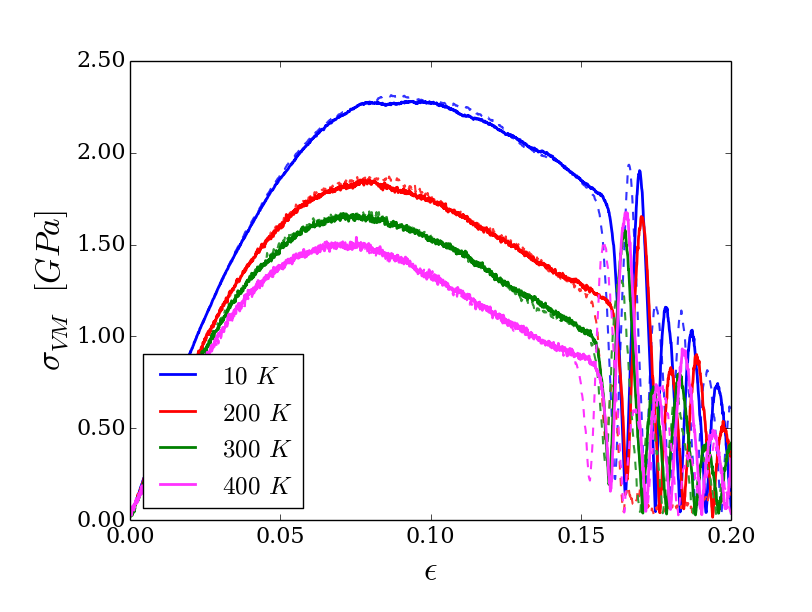
\includegraphics[width=6.3cm]{Cap_4/stress_strain_tension_FCC_NoInc.png}}
	\subfloat[Compresi\'on]{
	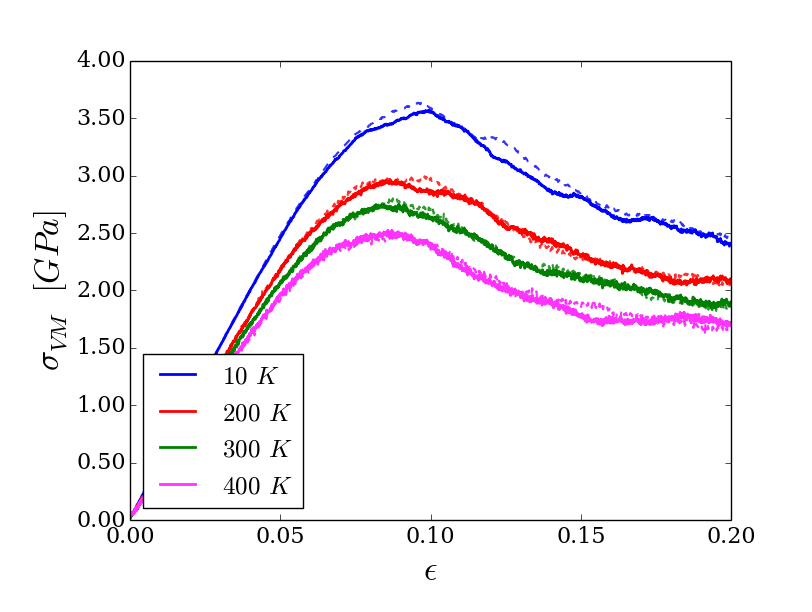
\includegraphics[width=6.3cm]{Cap_4/stress_strain_compression_FCC_NoInc.png}}
      \end{figure}
    \end{textblock*}
    \begin{textblock*}{12cm}(0.5cm,8.2cm) 
    \centering
      Tensi\'on de Von Mises vs deformaci\'on para el BMG sin inclusi\'on (l\'inea punteada) y una inclusi\'on de Cu-FCC (l\'inea s\'olida)
    \end{textblock*}
\end{frame}
\begin{frame}
  \frametitle{Carga uniaxial del BMG}
    \begin{textblock*}{12.6cm}(-0.08cm,1.5cm) 
      \begin{figure}[htp]
	\centering
	\subfloat[Tracci\'on]{
	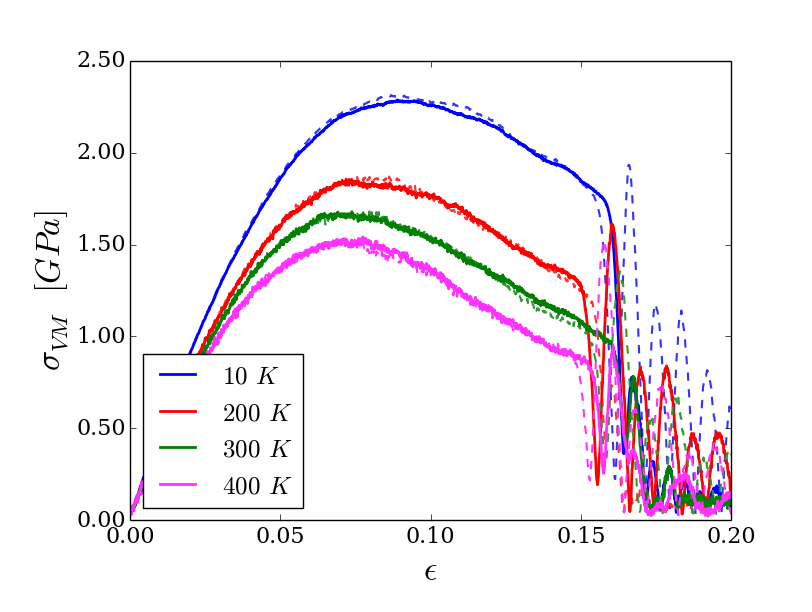
\includegraphics[width=6.3cm]{Cap_4/stress_strain_tension_B2_NoInc.png}}
	\subfloat[Compresi\'on]{
	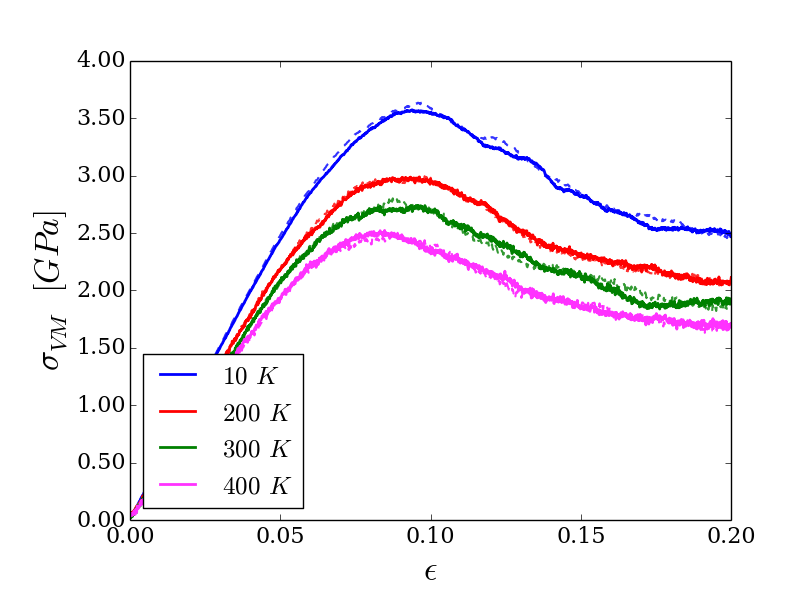
\includegraphics[width=6.3cm]{Cap_4/stress_strain_compression_B2_NoInc.png}}
      \end{figure}
    \end{textblock*}
    \begin{textblock*}{12cm}(0.5cm,8.2cm) 
    \centering
      Tensi\'on de Von Mises vs deformaci\'on para el BMG sin inclusi\'on (l\'inea punteada) y una inclusi\'on de CuZr-B2 (l\'inea s\'olida)
    \end{textblock*}
\end{frame}

\begin{frame}
  \frametitle{Cortes de la muestra}
  \begin{textblock*}{12.6cm}(-0.08cm,1.5cm) 
    \begin{figure}[htp]
     \centering
     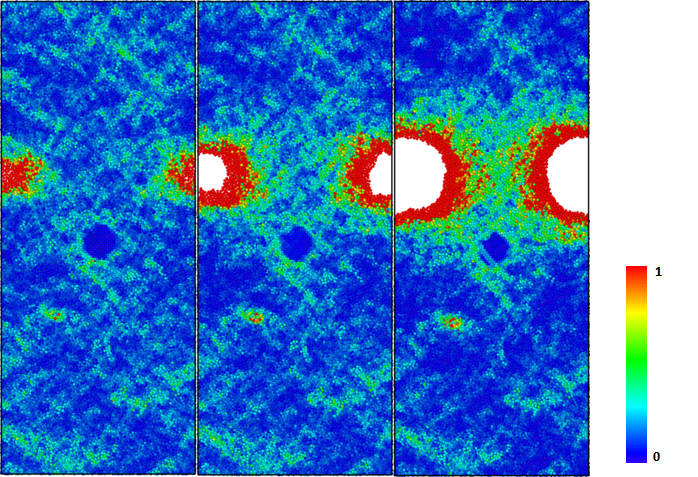
\includegraphics[height=6cm]{../Presentacion/Nanoparticles/cuSphereTension_10K_Snapshots.png}
    \end{figure}
  \end{textblock*}
  \begin{textblock*}{12cm}(0.5cm,8.5cm) 
    \centering
      \small{Inclusi\'on de Cu-FCC bajo tracci\'on a 10K según deformaci\'on atómica. De izquierda a derecha: $\epsilon$ = 16.66 \%, 16.68 \% y 16.70 \%.}
    \end{textblock*}

   \only<2>{
    \begin{textblock*}{10cm}(6cm,2cm)
      \begin{figure}[htp]
	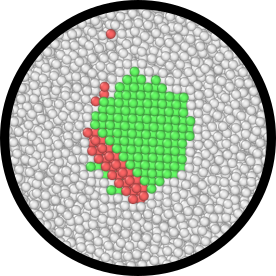
\includegraphics[width=3cm]{Presentacion/nanoparticles_macla.png}
    \end{figure}
    \end{textblock*}
    \begin{textblock*}{6cm}(8.4cm,5.3cm)
     \begin{tikzpicture}[overlay]
      \path[line width=0.8mm,fill=black,solid,<-] (0,0) edge [bend right] (1.4,0.4);
      \end{tikzpicture}
    \end{textblock*}
    

   }
\end{frame}

\begin{frame}
  \frametitle{Cortes de la muestra}
  \begin{textblock*}{12.6cm}(-0.08cm,1.5cm) 
    \begin{figure}[htp]
     \centering
     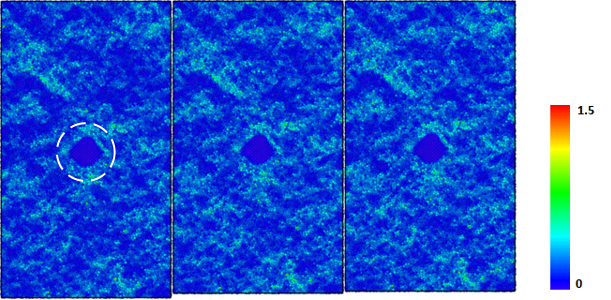
\includegraphics[height=6cm]{../Presentacion/Nanoparticles/cuSphereCompression_10K_Snapshots.png}
    \end{figure}
  \end{textblock*}
  \begin{textblock*}{12cm}(0.5cm,8.5cm) 
    \centering
      \small{Inclusi\'on de Cu-FCC bajo compresi\'on a 10K según deformaci\'on atómica. De izquierda a derecha: $\epsilon$ = 16.74 \%, 16.86 \% y 16.92 \%.}
    \end{textblock*}
\end{frame}

\begin{frame}
  \frametitle{Cortes de la muestra}
  \begin{textblock*}{12.6cm}(-0.08cm,1.5cm) 
    \begin{figure}[htp]
     \centering
     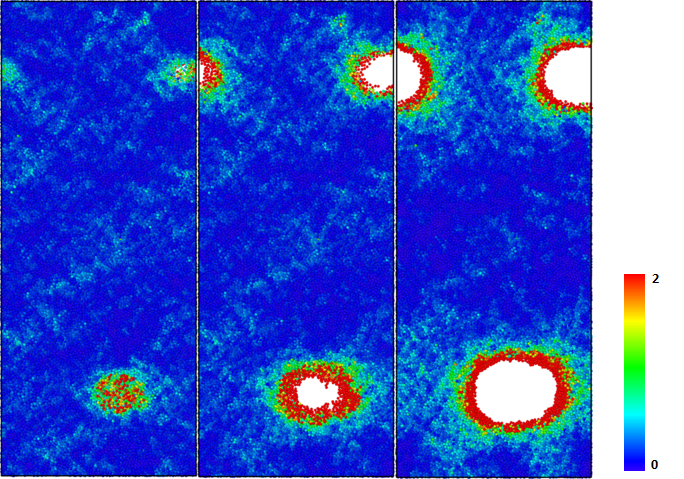
\includegraphics[height=6cm]{../Presentacion/Nanoparticles/B2SphereTension_10K_Snapshots.png}
    \end{figure}
  \end{textblock*}
  \begin{textblock*}{12cm}(0.5cm,8.5cm) 
    \centering
      \small{Inclusión de CuZr-B2 bajo tracción a 10K según deformación atómica. De izquierda a derecha: $\epsilon$ = 16.66 \%, 16.68 \% y 16.70 \%.}
    \end{textblock*}
\end{frame}

\begin{frame}
  \frametitle{Cortes de la muestra}
  \begin{textblock*}{12.6cm}(-0.08cm,1.5cm) 
    \begin{figure}[htp]
     \centering
     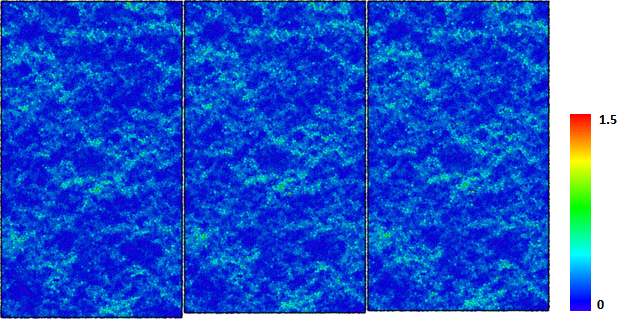
\includegraphics[height=6cm]{../Presentacion/Nanoparticles/B2SphereCompression_10K_Snapshots.png}
    \end{figure}
  \end{textblock*}
  \begin{textblock*}{12cm}(0.5cm,8.5cm) 
    \centering
      \small{Inclusión de CuZr-B2 bajo compresión a 10K según deformación atómica. De izquierda a derecha: $\epsilon$ = 16.74 \%, 16.86 \% y 16.92 \%.}
    \end{textblock*}
\end{frame}


%%%%%%%%%%%%%%%%%%%%%%%%%%%%%%%%%%%%%%%%%%%%%%%%%%%%%
%		CAP 5
%%%%%%%%%%%%%%%%%%%%%%%%%%%%%%%%%%%%%%%%%%%%%%%%%%%%%

\section[BMG poroso]{BMG poroso sinterizado}
%\subsection{BMG poroso sinterizado}
%%%
% Introduccion
%%%

\begin{frame}
    \frametitle{Introduction}
    \vspace{0.2cm}
    \begin{itemize}
        \item Metallic Glass: amorphous metal (without crystalline order).
        \item Has advantages over crystalline metals, like elasticity combined with high resistance, strength and moldability.
        \item Plasticity in these materials occurs by nucleation of shear transformation zones which grow into shear bands.
        \item Shear bands may lead to brittle failure (heterogeneous deformation): importance of \textbf{preventing their propagation}.
        \item A more homogeneous deformation may be achieved by adding \textbf{porosity}.
    \end{itemize} 
\end{frame}

\note{
    \begin{textblock*}{11.5cm}(0.5cm,2.5cm) 
        \begin{itemize}
            \item Example applications for MGs: amorphous structural steels, biomedical materials, aerospace materials, etc.
            \item Production of MGs: techniques which include high quenching rates, low volumes and composition control.
            \item STZs and SBs: STZs are small zones of intense shearing strain, consisting of a few atoms. A SB contains more atoms and has a different aspect ratio.
            \item Porosity to evitate the propagation of SBs: related to the way of preventing dislocation motion in metals.
            \item MD (Molecular Dynamics): solves problems with many atoms, interacting through an interatomic potential or force field.
        \end{itemize} 
    \end{textblock*}
 }

%%%
% Detalles de la simulacion
%%%

\begin{frame}
    \frametitle{Simulation details}
    \vspace{0.2cm}
    \begin{itemize}
        \item Software: Lammps (lammps.sandia.gov) for simulation, Ovito (www.ovito.org) and Gnuplot for analysis.
        \item Sample: based on Cu$_{46}$ Zr$_{54}$ described by Arman et al. (2010).
        \begin{itemize}
            \item Cooling rate 10$^{12}$ K/s.
        \end{itemize}
        \item EAM (Embedded Atom Method; Daw, 1984) alloy potential adopted (Cheng, 2008).
    \end{itemize}
    \begin{textblock*}{12cm}(0.5cm,7.5cm) % {block width} (coords)
        \scriptsize{Arman B., Luo S.-N., Germann T.C. and Cağin T., \textit{Phys. Rev. B.}, \textbf{81}, 144201 (2010).\\
        Daw M. and Baskes M.I., \textit{Phys. Rev. B.}, \textbf{29}:6443-6453 (1984).\\
        Cheng Y.Q., Sheng H.W. and Ma E., \textit{Phys. Rev. B.}, \textbf{78}, 014207 (2008) https://sites.google.com/site/eampotentials/}
    \end{textblock*}
\end{frame}

\note{
    \begin{textblock*}{12cm}(0.5cm,6.5cm) 
      EAM: the total energy $E_i$ of an atom $i$ is given by this equation, where F is the embedding energy which is a function of the atomic electron density $\rho$, $\phi$ is a pair potential interaction, and $\alpha$ and $\beta$ are the element types of atoms I and J. The multi-body nature of the EAM potential is a result of the embedding energy term. Both summations in the formula are over all neighbors J of atom I within the cutoff distance.
    \end{textblock*}
    \begin{block}{EAM}
        \[
            E_i=F_{\alpha} \left ( \sum \limits_{i\neq j} \rho _{\beta} (r_{ij}) \right ) + \frac{1}{2} \sum \limits_{i\neq j} \phi _{\alpha \beta} (r_{ij})
        \]
    \end{block}
}

%%%
% Preparacion de la muestra
%%%

\begin{frame}
    \frametitle{Porous sample preparation}
    \framesubtitle{Procedure}
    \vspace{0cm}
    \begin{enumerate}
        \item Random placement of 2.5 nm radius spheres.
        \item Relaxation @ 650K (constant volume, few ps). 
        \item Up to 10 ps of compressive pressure (400 bar).
        \item Repeat two previous steps.
        \item Further relaxation: cooling to zero T, barostat to zero pressure, heating to simulation temperature and, barostat to zero pressure (5 ps, constant T)
        \begin{textblock*}{3cm}(2.5cm,6.5cm) % {block width} (coords)
            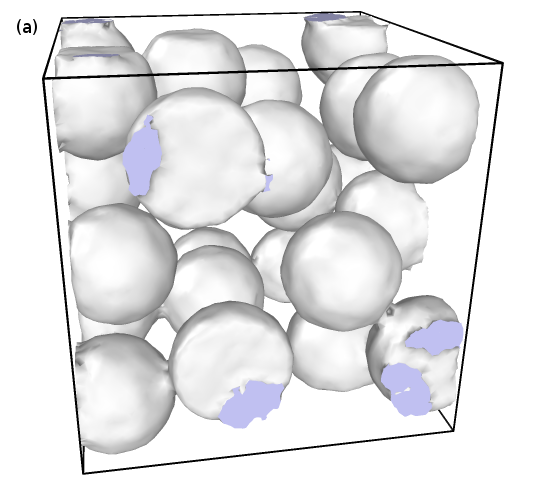
\includegraphics[width=3cm]{Presentacion_PANACM_Franco/spheres2.png}
        \end{textblock*}
        \begin{textblock*}{3cm}(7cm,6.5cm) % {block width} (coords)
            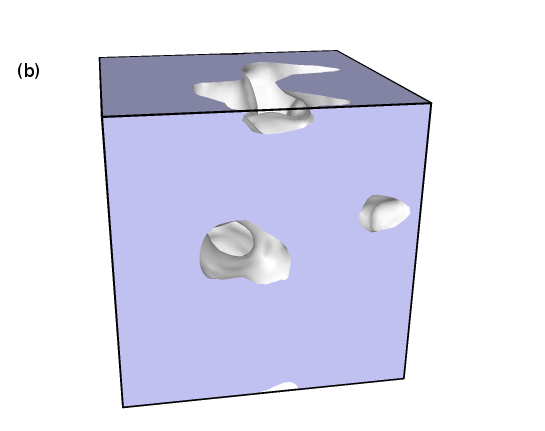
\includegraphics[width=3cm]{Presentacion_PANACM_Franco/spheres3.png}
        \end{textblock*}
    \end{enumerate}
\end{frame}

%%%
% Resultados
%%%

\begin{frame}
    \frametitle{Results}
    \framesubtitle{Samples and loading}
    \vspace{1cm}
    \begin{itemize}
        \item Took samples of different initial porosities (3.3\%, 5.8\% and 13.1\%).
        \item Loading at a strain rate of 10$^9/s$, appropiate for shock compression experiments.
        \item Purely uniaxial strain.
        \item Periodic boundary conditions.
    \end{itemize}
\end{frame}

\begin{frame}
    \frametitle{Results}
    \framesubtitle{Compression}
    \begin{textblock*}{7.5cm}(0.3cm,2cm) % {block width} (coords)
        \includegraphics[width=7.5cm]{Presentacion_PANACM_Franco/Pzz_strain_comp_dash.eps}
    \end{textblock*}
    \begin{textblock*}{4.2cm}(0.6cm,6.75cm) % {block width} (coords)
        \begin{tikzpicture}
            \draw[thick] (0,0) rectangle (5cm,1.2cm);
        \end{tikzpicture}
    \end{textblock*}
    \begin{textblock*}{5cm}(7.86cm,2.5cm) % {block width} (coords)
        After pore closure, curves are similar to the one for no porosity. There is significant hardening after pore closure.
    \end{textblock*}
    \begin{textblock*}{5cm}(7.86cm,5.8cm) % {block width} (coords)
        Before pore closure, strain increases while maintaining low stress levels.\\
        Porosity produces shear concentration, and pores start to collapse.
    \end{textblock*}
\end{frame}

\begin{frame}
    \frametitle{Results}
    \framesubtitle{Compression}
    \begin{textblock*}{6.5cm}(0.4cm,2cm) % {block width} (coords)
        \includegraphics[width=4cm]{Presentacion_PANACM_Franco/13_0strain.png}
        \includegraphics[width=4cm]{Presentacion_PANACM_Franco/13_5strain_comp.png}
        \includegraphics[width=4cm]{Presentacion_PANACM_Franco/13_12strain_comp.png}
    \end{textblock*}
    \begin{textblock*}{11cm}(1.2cm,6.4cm) % {block width} (coords)
        \centering
        \tiny{Shear strain coloring for a thin slice of the 13\% porosity sample. Strains are 0, 5 and 12\%\\Blue correspondes to shear strain lower than 10\%, and red to shear strain greater than 30\%}
    \end{textblock*}
    \begin{textblock*}{11cm}(1cm,7.1cm) % {block width} (coords)
        Pores act as stress concentrators.\\
        They also impede incipient shear band formation.\\
        Accumulation of strain along diagonal directions, as in incipient shear banding.
    \end{textblock*}
\end{frame}

\begin{frame}
    \frametitle{Results}
    \framesubtitle{Compression}
    \begin{textblock*}{7.5cm}(0.3cm,2cm) % {block width} (coords)
        \includegraphics[width=7.5cm]{Presentacion_PANACM_Franco/tipe3_strain_comp.eps}
    \end{textblock*}
    \begin{textblock*}{5cm}(7.9cm,2.5cm) % {block width} (coords)
        The fall in the number of Type 3 atoms after a constant stage has been thought to be an indicator of the onset of plasticity (Arman, 2010).
    \end{textblock*}
    \begin{textblock*}{5cm}(8cm,5.8cm) % {block width} (coords)
        Counter-intuitive result.\\
        Here we do have plasticity but there is almost no change in Voronoi polyhedra.\\
        Other processes involved?
    \end{textblock*}
\end{frame}

\note{
    \begin{textblock*}{6.5cm}(2.5cm,2.5cm) % {block width} (coords)
        \includegraphics[width=6.5cm]{Presentacion_PANACM_Franco/SVF_strain_comp_dash.eps}
    \end{textblock*}
    \begin{textblock*}{3cm}(9.2cm,3cm) % {block width} (coords)
        Solid volume fraction versus strain.
    \end{textblock*}
    \begin{textblock*}{9cm}(2.8cm,7.9cm) % {block width} (coords)
        The dashed lines show when pores totally close. The values are: \\
        $3\% \rightarrow 0.05, 6\% \rightarrow 0.065, 13\% \rightarrow 0.12$
    \end{textblock*}
}

\note{
    \begin{textblock*}{6.5cm}(2.5cm,2.5cm) % {block width} (coords)
        \includegraphics[width=6.5cm]{Presentacion_PANACM_Franco/stress_strain_comp_dash.eps}
    \end{textblock*}
    \begin{textblock*}{3cm}(9.2cm,3cm) % {block width} (coords)
        Von Mises stress versus strain.
    \end{textblock*}
    \begin{textblock*}{9cm}(2.8cm,8.2cm) % {block width} (coords)

    \end{textblock*}
}

\begin{frame}
    \frametitle{Results}
    \framesubtitle{Tension}
    \begin{textblock*}{7.5cm}(0.3cm,2cm) % {block width} (coords)
        \includegraphics[width=7.5cm]{Presentacion_PANACM_Franco/Pzz_strain_tens.eps}
    \end{textblock*}
    \begin{textblock*}{4cm}(8cm,2.2cm) % {block width} (coords)
        \includegraphics[width=4cm]{Presentacion_PANACM_Franco/13_20strain_tens.png}\\
        \centering
        \tiny{Shear strain coloring of the 13\% porosity sample’s slice at 20\% strain.}
    \end{textblock*}
    \begin{textblock*}{11.5cm}(0.5cm,7.8cm) % {block width} (coords)
        Plastic flow.\\
        The use of periodic boundary conditions precludes the closing of the voids (there is no necking).
    \end{textblock*}
\end{frame}

\begin{frame}
    \frametitle{Results}
    \framesubtitle{Tension}
    \begin{textblock*}{6.5cm}(0.4cm,2cm) % {block width} (coords)
        \includegraphics[width=4cm]{Presentacion_PANACM_Franco/13_0strain.png}
        \includegraphics[width=4cm]{Presentacion_PANACM_Franco/13_6strain_tens.png}
        \includegraphics[width=4cm]{Presentacion_PANACM_Franco/13_20strain_tens_2.png}
    \end{textblock*}
    \begin{textblock*}{11cm}(1cm,7cm) % {block width} (coords)
        \centering
        \tiny{Shear strain coloring of a thin slice of the 13\% porosity sample. Strains are 0, 6 and 20\%\\Blue correspondes to shear strain lower than 10\%, and red to shear strain greater than 30\%}
    \end{textblock*}
    \begin{textblock*}{11.5cm}(1cm,8cm) % {block width} (coords)
        Shear strain is mostly concentrated around the pores.
%            \item Relative position between atoms remains almost the same.
    \end{textblock*}
\end{frame}

\begin{frame}
    \frametitle{Results}
    \framesubtitle{Tension}
    \begin{textblock*}{7.5cm}(0.3cm,2cm) % {block width} (coords)
        \includegraphics[width=7.5cm]{Presentacion_PANACM_Franco/tipe3_strain_tens.eps}
    \end{textblock*}
    \begin{textblock*}{4.2cm}(6.7cm,4cm) % {block width} (coords)
        \begin{tikzpicture}
            \draw[thick] (0,0) rectangle (1.4cm,2cm);
        \end{tikzpicture}
    \end{textblock*}
    \begin{textblock*}{5cm}(8cm,3cm) % {block width} (coords)
        Constant after void nucleation.
    \end{textblock*}
    \begin{textblock*}{12cm}(0.4cm,7.9cm) % {block width} (coords)
        There is significant motion of atoms around pores, preventing the formation of STZs other than the ones around the pores.
    \end{textblock*}
\end{frame}

\note{
    \begin{textblock*}{6.5cm}(2.5cm,2.5cm) % {block width} (coords)
        \includegraphics[width=6.5cm]{Presentacion_PANACM_Franco/SVF_strain_tens.eps}
    \end{textblock*}
    \begin{textblock*}{3cm}(9.2cm,3cm) % {block width} (coords)
        Solid volume fraction versus strain.
    \end{textblock*}
}

\note{
    \begin{textblock*}{6.5cm}(2.5cm,2.5cm) % {block width} (coords)
        \includegraphics[width=6.5cm]{Presentacion_PANACM_Franco/stress_strain_tens.eps}
    \end{textblock*}
    \begin{textblock*}{3cm}(9.2cm,3cm) % {block width} (coords)
        Von Mises stress versus strain.
    \end{textblock*}
    \begin{textblock*}{9cm}(2.8cm,8.2cm) % {block width} (coords)

    \end{textblock*}
}

%%%
% Conclusiones
%%%

\begin{frame}
    \frametitle{Conclusions}
    \vspace{0.5cm}
    \begin{itemize}
        \item Sintering process leads to glass with taylored porosity values.
        \item Under compression: pores act as stress concentrators but also delay nucleation of SBs. After closure, there is hardening.
        \item Under tension: pores do not close and they concentrate plastic flow around them, also impeding formation of STZ and SBs.
        \item Results under strain were somewhat comparable to the ones by Yuan et al. (2014), where a single crystal sample with voids was studied.
    \end{itemize}
    \begin{textblock*}{12cm}(1cm,8.8cm) % {block width} (coords)
        \scriptsize{Yuan F. and Wu X., \textit{AIP ADVANCES}, \textbf{4}, 127109 (2014).}
    \end{textblock*}
\end{frame}

\note{
    \begin{textblock*}{5cm}(2cm,3.2cm) % {block width} (coords)
        \includegraphics[width=5cm]{Presentacion_PANACM_Franco/stress_strain_comp_dash.eps}
    \end{textblock*}
    \begin{textblock*}{3cm}(7cm,3cm) % {block width} (coords)
        \includegraphics[width=5cm]{Presentacion_PANACM_Franco/Yuan_VM.png}
    \end{textblock*}
    \begin{textblock*}{12cm}(1cm,8.2cm) % {block width} (coords)
        \small{Yuan F. and Wu X., \textit{AIP ADVANCES}, \textbf{4}, 127109 (2014).}
    \end{textblock*}
}

\note{
    \begin{textblock*}{5cm}(2cm,3.2cm) % {block width} (coords)
        \includegraphics[width=5cm]{Presentacion_PANACM_Franco/SVF_strain_comp_dash.eps}
    \end{textblock*}
    \begin{textblock*}{3cm}(7cm,3cm) % {block width} (coords)
        \includegraphics[width=5cm]{Presentacion_PANACM_Franco/Yuan_SVF.png}
    \end{textblock*}
    \begin{textblock*}{12cm}(1cm,8.2cm) % {block width} (coords)
        \small{Yuan F. and Wu X., \textit{AIP ADVANCES}, \textbf{4}, 127109 (2014).}
    \end{textblock*}
}
%%%%%%%%%%%%%%%%%%%%%%%%%%%%%%%%%%%%%%%%%%%%%%%%%%%%%%
%		APENDICES
%%%%%%%%%%%%%%%%%%%%%%%%%%%%%%%%%%%%%%%%%%%%%%%%%%%%%

\section{Trabajo computacional}
%\subsection{Trabajo computacional}

\begin{frame}
 
\end{frame}
%%%%%%%%%%%%%%%%%%%%%%%%%%%%%%%%%%%%%%%%%%%%%%%%%%%%%
%		CONCLUSIONES
%%%%%%%%%%%%%%%%%%%%%%%%%%%%%%%%%%%%%%%%%%%%%%%%%%%%%

\section{Conclusiones}
\subsection{Conclusiones}

\begin{frame}
  \frametitle{CONCLUSIONES}
  \vspace{0.3cm}
 \begin{itemize} 
  \item Se aproxima el comportamiento en función de la temperatura con una función de decaimiento exponencial. No se encuentran trabajos en la literatura que realicen estas aproximaciones.
  \vspace{0.3cm}
  \item Se observa una marcada asimetría tracción - compresión. Pocos trabajos analizan distintos tipos de carga.
  \vspace{0.3cm}
  \item Se observan bandas de corte, las cuales son más evidentes con condiciones de frontera libre.
  \end{itemize}
\end{frame}

\begin{frame}
  \frametitle{CONCLUSIONES}
  \vspace{0.6cm}
 \begin{itemize} 
  \item Analizamos los efectos de la temperatura sobre nanopartículas embebidas, indicando estabilidad debajo de 400 K. A temperaturas más elevadas, se pierde la frontera nítida cristal/amorfo.
  \vspace{0.6cm}
  \item Las curvas tensión-deformación de la matriz con inclusión son muy similares al caso sin nanopartícula, pero existe un retardo en la nucleación de poros bajo tracción.
 \end{itemize}
\end{frame}

\begin{frame}
  \frametitle{CONCLUSIONES}
  \vspace{1cm}
 \begin{itemize}
  \item Muestra porosa bajo compresión: los poros concentran tensiones pero también retrasan la nucleación de SBs.
  \vspace{1cm}
  \item Muestra porosa bajo tracción: los poros no se cierran y facilitan el movimiento de átomos a su alrededor, impidiendo la formación de STZs y SBs.
 \end{itemize}
\end{frame}

\begin{frame}
 \frametitle{PRESENTACIONES EN CONGRESOS}
 \vspace{0.2cm}
 \begin{itemize}
  \item Trabajo completo publicado y presentado en el X Congreso Argentino de Mecánica Computacional (MECOM 2012)
  \vspace{0.2cm}
  \item Dos trabajos completos publicados y presentados en el I Congreso Panamericano de Mecánica Computacional (PANACM 2015)
 \end{itemize}
  \vspace{0.5cm}
  Además, se presentaron posters de estudiantes en el X Congreso Argentino de Mecánica Computacional (MECOM 2012) 
\end{frame}


\begin{frame}
 \frametitle{Trabajos futuros}
 \vspace{0.3cm}
 \begin{itemize}
  \item Generar y estudiar muestras a menores velocidades de enfriamiento y velocidad de deformación.
  \vspace{0.4cm}
  \item Estudiar muestras de mayor tamaño (mayor cantidad de nanopartículas y diferentes topologías de poros).
  \vspace{0.4cm}
  \item Llevar propiedades del estudio nano a códigos de elementos finitos para estudiar piezas de mayor tamaño.
  \vspace{0.4cm}
  \item Investigar el origen de la asimetría tracción - compresión.
 \end{itemize}
\end{frame}


%\section{Bibliografía}
%\begin{frame}
%  \tiny{\bibliographystyle{apalike}}
  \bibliography{../Bibliography}
%\end{frame}

%%%
% Slide de titulo
%%%

\maketitle

\end{document}
